% Options for packages loaded elsewhere
\PassOptionsToPackage{unicode}{hyperref}
\PassOptionsToPackage{hyphens}{url}
\PassOptionsToPackage{dvipsnames,svgnames,x11names}{xcolor}
%
\documentclass[
  letterpaper,
  DIV=11,
  numbers=noendperiod]{scrartcl}

\usepackage{amsmath,amssymb}
\usepackage{iftex}
\ifPDFTeX
  \usepackage[T1]{fontenc}
  \usepackage[utf8]{inputenc}
  \usepackage{textcomp} % provide euro and other symbols
\else % if luatex or xetex
  \usepackage{unicode-math}
  \defaultfontfeatures{Scale=MatchLowercase}
  \defaultfontfeatures[\rmfamily]{Ligatures=TeX,Scale=1}
\fi
\usepackage{lmodern}
\ifPDFTeX\else  
    % xetex/luatex font selection
\fi
% Use upquote if available, for straight quotes in verbatim environments
\IfFileExists{upquote.sty}{\usepackage{upquote}}{}
\IfFileExists{microtype.sty}{% use microtype if available
  \usepackage[]{microtype}
  \UseMicrotypeSet[protrusion]{basicmath} % disable protrusion for tt fonts
}{}
\makeatletter
\@ifundefined{KOMAClassName}{% if non-KOMA class
  \IfFileExists{parskip.sty}{%
    \usepackage{parskip}
  }{% else
    \setlength{\parindent}{0pt}
    \setlength{\parskip}{6pt plus 2pt minus 1pt}}
}{% if KOMA class
  \KOMAoptions{parskip=half}}
\makeatother
\usepackage{xcolor}
\setlength{\emergencystretch}{3em} % prevent overfull lines
\setcounter{secnumdepth}{5}
% Make \paragraph and \subparagraph free-standing
\ifx\paragraph\undefined\else
  \let\oldparagraph\paragraph
  \renewcommand{\paragraph}[1]{\oldparagraph{#1}\mbox{}}
\fi
\ifx\subparagraph\undefined\else
  \let\oldsubparagraph\subparagraph
  \renewcommand{\subparagraph}[1]{\oldsubparagraph{#1}\mbox{}}
\fi


\providecommand{\tightlist}{%
  \setlength{\itemsep}{0pt}\setlength{\parskip}{0pt}}\usepackage{longtable,booktabs,array}
\usepackage{calc} % for calculating minipage widths
% Correct order of tables after \paragraph or \subparagraph
\usepackage{etoolbox}
\makeatletter
\patchcmd\longtable{\par}{\if@noskipsec\mbox{}\fi\par}{}{}
\makeatother
% Allow footnotes in longtable head/foot
\IfFileExists{footnotehyper.sty}{\usepackage{footnotehyper}}{\usepackage{footnote}}
\makesavenoteenv{longtable}
\usepackage{graphicx}
\makeatletter
\def\maxwidth{\ifdim\Gin@nat@width>\linewidth\linewidth\else\Gin@nat@width\fi}
\def\maxheight{\ifdim\Gin@nat@height>\textheight\textheight\else\Gin@nat@height\fi}
\makeatother
% Scale images if necessary, so that they will not overflow the page
% margins by default, and it is still possible to overwrite the defaults
% using explicit options in \includegraphics[width, height, ...]{}
\setkeys{Gin}{width=\maxwidth,height=\maxheight,keepaspectratio}
% Set default figure placement to htbp
\makeatletter
\def\fps@figure{htbp}
\makeatother
\newlength{\cslhangindent}
\setlength{\cslhangindent}{1.5em}
\newlength{\csllabelwidth}
\setlength{\csllabelwidth}{3em}
\newlength{\cslentryspacingunit} % times entry-spacing
\setlength{\cslentryspacingunit}{\parskip}
\newenvironment{CSLReferences}[2] % #1 hanging-ident, #2 entry spacing
 {% don't indent paragraphs
  \setlength{\parindent}{0pt}
  % turn on hanging indent if param 1 is 1
  \ifodd #1
  \let\oldpar\par
  \def\par{\hangindent=\cslhangindent\oldpar}
  \fi
  % set entry spacing
  \setlength{\parskip}{#2\cslentryspacingunit}
 }%
 {}
\usepackage{calc}
\newcommand{\CSLBlock}[1]{#1\hfill\break}
\newcommand{\CSLLeftMargin}[1]{\parbox[t]{\csllabelwidth}{#1}}
\newcommand{\CSLRightInline}[1]{\parbox[t]{\linewidth - \csllabelwidth}{#1}\break}
\newcommand{\CSLIndent}[1]{\hspace{\cslhangindent}#1}

\usepackage{booktabs}
\usepackage{longtable}
\usepackage{array}
\usepackage{multirow}
\usepackage{wrapfig}
\usepackage{float}
\usepackage{colortbl}
\usepackage{pdflscape}
\usepackage{tabu}
\usepackage{threeparttable}
\usepackage{threeparttablex}
\usepackage[normalem]{ulem}
\usepackage{makecell}
\usepackage{xcolor}
\usepackage{cancel}
\addtokomafont{disposition}{\rmfamily}
\KOMAoption{captions}{tableheading}
\makeatletter
\makeatother
\makeatletter
\makeatother
\makeatletter
\@ifpackageloaded{caption}{}{\usepackage{caption}}
\AtBeginDocument{%
\ifdefined\contentsname
  \renewcommand*\contentsname{Table of contents}
\else
  \newcommand\contentsname{Table of contents}
\fi
\ifdefined\listfigurename
  \renewcommand*\listfigurename{List of Figures}
\else
  \newcommand\listfigurename{List of Figures}
\fi
\ifdefined\listtablename
  \renewcommand*\listtablename{List of Tables}
\else
  \newcommand\listtablename{List of Tables}
\fi
\ifdefined\figurename
  \renewcommand*\figurename{Figure}
\else
  \newcommand\figurename{Figure}
\fi
\ifdefined\tablename
  \renewcommand*\tablename{Table}
\else
  \newcommand\tablename{Table}
\fi
}
\@ifpackageloaded{float}{}{\usepackage{float}}
\floatstyle{ruled}
\@ifundefined{c@chapter}{\newfloat{codelisting}{h}{lop}}{\newfloat{codelisting}{h}{lop}[chapter]}
\floatname{codelisting}{Listing}
\newcommand*\listoflistings{\listof{codelisting}{List of Listings}}
\usepackage{amsthm}
\theoremstyle{plain}
\newtheorem{proposition}{Proposition}[section]
\theoremstyle{plain}
\newtheorem{corollary}{Corollary}[section]
\theoremstyle{remark}
\AtBeginDocument{\renewcommand*{\proofname}{Proof}}
\newtheorem*{remark}{Remark}
\newtheorem*{solution}{Solution}
\makeatother
\makeatletter
\@ifpackageloaded{caption}{}{\usepackage{caption}}
\@ifpackageloaded{subcaption}{}{\usepackage{subcaption}}
\makeatother
\makeatletter
\@ifpackageloaded{tcolorbox}{}{\usepackage[skins,breakable]{tcolorbox}}
\makeatother
\makeatletter
\@ifundefined{shadecolor}{\definecolor{shadecolor}{rgb}{.97, .97, .97}}
\makeatother
\makeatletter
\makeatother
\makeatletter
\makeatother
\ifLuaTeX
  \usepackage{selnolig}  % disable illegal ligatures
\fi
\IfFileExists{bookmark.sty}{\usepackage{bookmark}}{\usepackage{hyperref}}
\IfFileExists{xurl.sty}{\usepackage{xurl}}{} % add URL line breaks if available
\urlstyle{same} % disable monospaced font for URLs
\hypersetup{
  pdftitle={The behavioral effects of index insurance in fisheries},
  pdfauthor={Nathaniel Grimes; Christopher Costello; Andrew J. Plantinga},
  pdfkeywords={Index Insurance, Moral Hazard, Fisheries, Conservation},
  colorlinks=true,
  linkcolor={blue},
  filecolor={Maroon},
  citecolor={Blue},
  urlcolor={Blue},
  pdfcreator={LaTeX via pandoc}}

\title{The behavioral effects of index insurance in fisheries}
\usepackage{etoolbox}
\makeatletter
\providecommand{\subtitle}[1]{% add subtitle to \maketitle
  \apptocmd{\@title}{\par {\large #1 \par}}{}{}
}
\makeatother
\subtitle{Working Paper Draft \emph{Not For Circulation}}
\author{Nathaniel Grimes \and Christopher Costello \and Andrew J.
Plantinga}
\date{2024-09-28}

\begin{document}
\maketitle
\begin{abstract}
Fisheries are vulnerable to environmental shocks that impact stock
health and fisher income. Index insurance is a promising financial tool
to protect fishers from environmental risk. However, insurance will
change fisher's behavior through moral hazards. We provide the first
theoretical application of index insurance on fisher's behavior change
to predict if index insurance will incentivize overfishing or
conservation of the stock. Using traditional fishery models will always
bias index insurance to incentivize overfishing, which in turn reduces
fish stocks. However, using models with more flexible input risk effects
shows index insurance will have varying effects on fishery conservation.
The direction of change depends on the risk characteristics of the
inputs. We find that index insurance will raise (lower) individual
fisher effort when effort is risk increasing (decreasing). In turn,
higher (lower) fishing effort reduces (increases) conservation of fish
stocks. The direction of harvest change becomes ambiguous when
accounting for interaction between multiple inputs. Simulating from
parameters estimated for four Norwegian fisheries shows index inusrance
could increase harvest as high as 15\% or decrease harvest by 6\%.
Before widespread adoption, careful consideration must be given to how
index insurance will incentivize or disincentivize overfishing.
\end{abstract}
\ifdefined\Shaded\renewenvironment{Shaded}{\begin{tcolorbox}[breakable, enhanced, sharp corners, borderline west={3pt}{0pt}{shadecolor}, interior hidden, frame hidden, boxrule=0pt]}{\end{tcolorbox}}\fi

\renewcommand*\contentsname{Table of contents}
{
\hypersetup{linkcolor=}
\setcounter{tocdepth}{3}
\tableofcontents
}
\hypertarget{introduction}{%
\section{Introduction}\label{introduction}}

Fisheries are vulnerable to stochastic weather shocks. Environmental
fluctuations directly impact fishers of all scales from large industrial
vessels to small scale subsistence fishers. Fishing is a vital economic
engine to coastal communities and is the primary source of protein for
millions of people (Sumaila \emph{et al.} 2012; Teh and Sumaila 2013;
FAO 2020). Supporting these communities requires protection from
enormous degrees of environmental risk.

Marine heatwaves provide a good example of how environmental variability
impacts fishery biological and economic productivity. Marine heatwaves
increase animal thermal stress diminishing reproductive ability
(Barbeaux \emph{et al.} 2020), stunting growth (Pandori and Sorte 2019),
pushing species outside their usual habitats (Cavole \emph{et al.}
2016), and may directly increase mortality (Smith \emph{et al.} 2023).
Expanding fish habitat ranges increase costs when moving beyond the
fishing grounds of established ports (Rogers \emph{et al.} 2019). The
variability from marine heatwaves alone impacts 77\% of species within
economic exclusion zones and reduces maximum catch potential by 6\%
(Cheung \emph{et al.} 2021). Marine heatwaves are often accompanied by
harmful algal blooms and diseases leading to additional fishery
collapses (Oken \emph{et al.} 2021).

The devastation of marine heatwaves was made clear in October 2022 when
the Alaskan snow crab fishery was shut down after an assessment revealed
an 87\% decline in population from 2018 (Zacher \emph{et al.} 2022). New
evidence suggests that the marine heatwave increased caloric demands
while tightening the snow crab range leading to a mass starvation event
(Szuwalski \emph{et al.} 2023). The fishery provided \$132 million from
landings and \$174 million from processing in 2020, and the impacts from
the closure will reverberate throughout the community (Garber-Yonts and
Lee 2022). Recorded marine heatwaves have become more frequent (Holbrook
\emph{et al.} 2019) and climate change may continue to increase heatwave
frequency as climate distributions become more variable (Frölicher
\emph{et al.} 2018).

Weather can also impact fisher harvesting efficiency beyond influencing
the health of the underlying stock. Rolling seas and high wind speeds
make it more difficult to harvest (Alvarez \emph{et al.} 2006) in
addition to raising the danger to crew and vessel (Heck \emph{et al.}
2021). More intense storms threaten coastal infrastructure vital to
fishing communities (Sainsbury \emph{et al.} 2019). Fishers actively
avoid fishing in destructive weather at the expense of lost income
(Pfeiffer 2020).

Individual choices by fishers and fishery management mitigate
environmental risk. However, there is a lack of financial tools
available to fishers to address income risk as a result of environmental
fluctuations (Sethi 2010; Kasperski and Holland 2013). There is growing
interest in developing new financial tools to alleviate financial and
income risk for coastal communities (Wabnitz and Blasiak 2019; Sumaila
\emph{et al.} 2020).

Insurance may be an ideal financial tool for risk management in
fisheries as it is scalable, protects against environmental shocks, and
smooths income for fishers (Watson \emph{et al.} 2023). Currently,
insurance in fisheries is primarily used to protect assets such as
vessel hulls or fishing gear (FAO 2022). Insurance coverage could be
expanded to include income variability. Weather fluctuations impact
fisher income and their livelihoods. An insurance product covering
environmental risk could improve fisher welfare and promote community
resilience (Maltby \emph{et al.} 2023).

Policy makers have begun pushing for new fisheries insurance programs
modeled after agricultural crop insurance programs (Murkowski 2022).
Index insurance is one such product touted by practitioners as a prime
candidate for fisheries productivity insurance (Watson \emph{et al.}
2023). Index insurance gained traction in agriculture as an effective
alternative to traditional crop insurance in developing countries
because it had lower administrative cost, minimized moral hazards, and
does not require claim verification (Collier \emph{et al.} 2009; Carter
\emph{et al.} 2017). Whereas indemnity crop insurance requires an
assessment of loss to an individual farm, index insurance uses an
independent measure as the basis for issuing payouts to all
policyholders. For example, a pilot program through the Caribbean Oceans
and Aqauculture Sustainability Facility (COAST) uses index insurance to
payout a set amount to fishers when indices of wave height, wind speed,
and storm surge indicate a hurricane (Sainsbury \emph{et al.} 2019).
Triggers are the index values that initiate a payout. Contract design
revolve around establishing suitable triggers to cover environmental
loss. Interest is growing in expanding index insurance to cover other
environmental shocks to more fisheries.

One crucial area that remains unaddressed is the potential influence of
insurance on fishers behavior. Moral hazards are decisions by insured
agents that they would not otherwise take if they were uninsured (Wu
\emph{et al.} 2020). Owning insurance contracts may change fisher
harvesting decisions through moral hazards, which could impact the
sustainability of fish stocks. Policy tools leveraging behavioral
changes have been used to promote environmental conservation of water,
energy, and fisheries (Campbell \emph{et al.} 2004; Reddy \emph{et al.}
2017; McDonald \emph{et al.} 2020). Index insurance could be used as a
tool to incentive sustainable behavior changes if the conditions are
right. However, no study has modeled or examined the behavioral
implications of a fisheries insurance program. Behavioral policies can
also backfire through unintended consequences especially in bio-economic
settings (Abbott and Haynie 2012). Therefore, it is imperative to have
some preemptive understanding of potential shortfalls of new policies.
Fisheries are highly dynamic systems because of year to year variation
in biological growth and reproduction stemming from environmental
variables. Overfishing impacts are exacerbated through ecological
dynamics as lower fish abundances carry over to the next year. With
35.6\% of global fisheries overfished and 57.3\% at maximum sustainable
yield (FAO 2022), ensuring new index insurance programs do not
incentivize perverse behavior towards more overfishing is a necessary
first assessment.

Previous studies articulated hypothetical examples of moral hazards in
fishery indemnity insurance programs, such as encouraging fishers to
fish in foul weather or to not exit the fishery after a bad year of
harvest (Herrmann \emph{et al.} 2004; Watson \emph{et al.} 2023).
Building a theoretical framework will better predict the long term
sustainability of index insurance programs for fisheries. Currently, the
operational assumption of practitioners appears to be that index
insurance would completely avoid any moral hazards in fisheries and
intrinsically motivate greater fishery sustainability {[}ORAA?{]}. Yet,
there are two components to insurance moral hazard: ``chasing the
trigger'' and ``risk reduction''. ``Chasing the trigger'' is the
directed behavior of policyholders to increase the likelihood of a
payout. For example, a fisher actively choosing to fish less to receive
an indemnified harvest insurance payment. Index insurance completely
eliminates this moral hazard through the independent and uninfluenced
index (fishers cannot affect sea surface temperature). ``Risk
reduction'' occurs through possessing an insurance contract that
protects policyholders from risk. Policyholders may reoptimize their
decisions once protected from risk. Index insurance remains susceptible
to this element of moral hazard that could manifest in maladaptive
behaviors. A simple example would be choosing to not wear a helmet while
riding a bike because you have health insurance. All preliminary
analyses of fisheries index insurance are missing rigorous assessment of
moral hazards. Moral hazards could enable behavior changes that lead to
conservation of fish stocks or spiral delicate systems towards
destruction.

Agricultural economists have grappled with insurance moral hazards for
decades. There are clear, demonstrable behavioral changes in farmers
because of insurance that impact environmental sustainability. Farmers
use more water (Deryugina and Konar 2017) and acreage with insurance
coverage (Goodwin \emph{et al.} 2004; Cai 2016; Claassen \emph{et al.}
2017). The direction of chemical input use varies with some studies
indicating increased fertilizer use (Horowitz and Lichtenberg 1993),
while others indicate less fertilizer use (Babcock and Hennessy 1996;
Smith and Goodwin 1996). Mishra \emph{et al.} (2005) were the first to
connect moral hazards to positive effects on the environment. Their
study found that reduced fertilizer use from insurance led to less
agricultural run-off pollution. Overall, insurance leads to
statistically significant changes in pollution levels, but are
proportionally rather small drivers of total agricultural pollution
(Claassen \emph{et al.} 2017).

Index insurance leads to changes in farmers behavior similar to those
observed in indemnity insurance. Index insurance increased agricultural
capital investments in Kenyan maize, Burkina Faso cotton, and Mali
cotton farmers (Elabed and Carter 2018; Sibiko and Qaim 2020; Stoeffler
\emph{et al.} 2022). Index insurance also encouraged farmers in India to
plant higher yield, but riskier crops (Cole \emph{et al.} (2017)). In
all instances, farmers took on riskier positions with the protection
offered by insurance; with each as clear demonstrations of the ``risk
reduction'' element in index insurance moral hazards.

Increased investments through insurance can also harm communities,
particularly in dynamic resources such as livestock grazing. Kenyan
index insurance for livestock discentivized preemptively selling animals
after negative shocks, leading to larger herds in aggregate, which in
turn reduce pasture health through overgrazing (Janzen and Carter 2018).
Though no empirical work has been done on the long term effects, two
theoretical studies suggest insurance increases the stocking levels of
grazing animals in pastures. Higher stocking densities diminish the
pasture's ecological long-term health reducing overall utility gains of
insurance (Müller \emph{et al.} 2011; Bulte and Haagsma 2021). Caution
must be demonstrated when dealing with complex bio-economic systems,
otherwise maladaptive outcomes can lead to greater harm (Müller \emph{et
al.} 2017). The race to fish incentive that leads to overexploitation is
a defining characteristic of fisheries. If index insurance always leads
to increased input use in common pool resources, then implementing index
insurance in fisheries could lead to maladaptive outcomes.

This paper explores how fishers could change their behavior if offered
viable index insurance contracts. We start in Section~\ref{sec-common}
with the canonical Gordon-Schaefer production model to show that
standard fishery models predict index insurance will always decrease
fish stocks leading to loss in abundance. If we adopt more flexible
production models, the effects of index insurance becomes ambiguous, and
may lead to healthier fish stocks. We parameterize a model to
demonstrate the potential impacts of index insurance. However, fishers
use multiple inputs while fishing. Therefore, we extend the theoretical
model to account for multiple inputs in Section~\ref{sec-multi} to
develop clearer insights with possible input interactions. Numerical
results in Section~\ref{sec-sim} estimate potential harvest changes with
an index insurance program. We calibrate an insurance model with input
estimates from Norwegian fisheries. Implications for the suitability of
fishery index insurance are discussed in Section~\ref{sec-disc}. Fishery
index insurance ultimately has ambiguous effects on conservation. Before
widespread adoption, careful consideration must be given to how
insurance will incentivize or disincentivize overfishing.

\hypertarget{sec-common}{%
\section{Index insurance with standard fishery
models}\label{sec-common}}

A set number of \(N\) fishers harvest from a common stock of fish.
Permits, limited entry policies, or geographic constraints could limit
\(N\) to be fixed. The fish stock, \(\tilde{B}\), is a random variable
that experiences stochastic shocks that directly changes the amount of
fish available for all fishers to harvest. We can separate the random
biomass variable into a mean effect, \(\hat{B}\), and a variance
component, \(\omega\), where \(\omega\) can have any distribution so
long as \(\mathbb{E}[\omega]=0\).

\begin{equation}\protect\hypertarget{eq-bio}{}{
\tilde{B}=\hat{B}+\omega
}\label{eq-bio}\end{equation}

This formulation is often referred to as process error, where randomness
could originate from weather shocks in the current period or measurement
error (Merino \emph{et al.} (2022);Tilman \emph{et al.} (2018)). An
individual fisher, \(i\), uses a vector of \(M\) inputs
\(X^i\in\{{x_1,x_2,...x_M}\}\) to harvest, \(y^i\), amount of fish. The
stock of fish also acts as an input to harvest
(\(y^i=f(X^i)\tilde{B}\)). All other fishers,
\(j \text{ where } j\ne i\), harvest from the same stock of fish with
their own vector of inputs, \(y^j=f(X^ j)\tilde{B}\). Aggregate harvest
of all other fishers accounts for every fishers' input vectors
\(Y(X^{\sim j})=\sum ^{N-1}_jy^j\). The lack of property rights and
competition between fishers leads to a subtractability externality.
Specifically, mean fish biomass (\(\hat{B}(X^i,Y(X^{\sim j}))\)) is
decreasing in aggregate harvest, \(\sum^{N}_{i=1} y^i\). Individual
fisher inputs may have different effects on mean production, \(f(X^i)\),
and the variance of production, \(h(X^i)\).

\begin{equation}\protect\hypertarget{eq-y}{}{
y^i=f(X^i)\hat{B}(X^i,Y(X^{\sim j}))+\omega h(X^i)
}\label{eq-y}\end{equation}

Fishers derive utility from profits and are price takers, so we add a
convex cost function to harvest and normalize price of harvest to 1.

\begin{equation}\protect\hypertarget{eq-pi1}{}{
\begin{aligned}
\pi^i=f(X^i)\hat{B}(X^i,Y(X^{\sim j}))+\omega h(X^i)-c(X^i)
\end{aligned}
}\label{eq-pi1}\end{equation}

To most seamlessly integrate index insurance, we create insurance
lotteries by defining a trigger, \(\bar\omega\), where insurance pays
out a constant amount \(\gamma\) if \(\omega<\bar\omega\). The
probability of entering a bad state and receiving the payout is
\(F(\bar\omega)\), where \(F(\omega)\) is the cumulative distribution of
\(\omega\). We can use \(\omega\) to create an index to indemnify
payouts because it captures the randomness of fishers' profits. In
reality, the index would be a weather variable known to impact biomass
such as sea surface temperature, and the trigger are critical thresholds
of the weather variable where biomass deviates significantly from the
mean. Here, all stochasticity is captured by \(\omega\) with no basis
risk.

Actuarilly fair insurance allows the premium, \(\rho\), paid in both
states to be the probability of receiving a payout times the payout
amount, \(\rho=F(\bar\omega)\gamma\). Additionally, if we set the
trigger to \(\bar\omega=0\) to indicate any time weather negatively
impacts production, profits will enter corresponding bad and good
states. This leads to the following corollary statement.

\begin{corollary}[]\protect\hypertarget{cor-mp}{}\label{cor-mp}

Individual fisher expected marginal profit of a specific input, \(x_m\),
is greater in the good state than expected marginal profit in the bad
state when \(h_{x_m}(X^i)>0\). Expected marginal profit is higher in the
bad state when \(h_{x_m}(X^i)<0\). If \(h_{x_m}(X^i)=0\), the marginal
profits are equivalent in both states.

\end{corollary}

The proof of Corollary~\ref{cor-mp} is included in the appendix.

Risk aversion is a necessary condition for insurance to be desirable
(Outreville 2014). Fishers are highly sensitive to risk, especially
income risk and demonstrate risk aversion despite working a seemingly
risky profession (Smith and Wilen 2005; Holland 2008; Sethi 2010). They
mitigate risk through a variety of measures. Fishers will choose
consistent, known fishing grounds over risking exploring unknown spots
(Holland 2008). Fishers choose to fish less after storms and hurricanes
when financial risk is alleviated by transitioning to catch share
programs (Pfeiffer 2020; Pfeiffer \emph{et al.} 2022). Therefore, we can
assume fishers are risk averse to income shocks through a concave
utility function. Fishers will maximize their own expected utility
across good and bad states by selecting inputs with an exogenous
insurance contract.

\begin{equation}\protect\hypertarget{eq-max}{}{
\begin{aligned}
U\equiv\max_{X^i}\mathbb{E}[U]=&F(\bar\omega)\mathbb{E}[u(\pi^i(X^i,\hat{B}(X^i,Y(X^{\sim j})),\omega)+(1-F(\bar\omega))\gamma|\omega<\bar\omega)]\\
&+(1-F(\bar\omega))\mathbb{E}[u(\pi^i(X^i,\hat{B}(X^i,Y(X^{\sim j})),\omega)-F(\bar\omega\gamma)|\omega>\bar\omega)]
\end{aligned}
}\label{eq-max}\end{equation}

The general model in Equation~\ref{eq-max} is a flexible framework that
can be applied to any fishery production model. A common characteristic
of fishery models is the use of a single input technology function that
increases with larger stocks of fish. Models of these forms include the
canonical Gordon-Schaefer model, the Pella-Tomlinson model,
(\textbf{Clark1975?}) in deterministic settings, and
(\textbf{Reed1979?}) for stochastic settings. However, all of these
models implicitly assume \(h^i_{x_m}(X^i)>0\). For example, the most
widespread fishing production function originates from the
Gordon-Schaefer model where
\(y^i=qx^i\tilde{B}(x^i,Y(x^{\sim j}))\)\footnote{Traditionally,
  Gordon-Schaefer uses \(e\) as the single input to denote aggregate
  fishing effort. To stay consistent with the terms used in this paper
  we present it as \(x^i\) for a single input}. Expanding the
stochasticity of biomass, production in Gordon-Schaefer becomes
\(y^i=q\hat{B}(x^iY(x^{\sim j}))x^i+\omega qx^i\). The derivative of the
risk component of the production function is always positive,
\(h_{x}(x^i)=q\), because the catchability coefficient \(q\) is positive
by definition.

We show how this implicit bias on risk production in canonical models
will always lead insurance to stimulate greater use of optimal inputs.
We simply the general model to one input to reflect the aggregate effort
used in these models.

\begin{proposition}[]\protect\hypertarget{prp-cp}{}\label{prp-cp}

Any single input fishery production model where \(h_{x}(x^i)>0\) will
always lead to increases in optimal input use with feasible index
insurance contracts.

\end{proposition}

\begin{proof}

Individual fishers now only use one input denoted by scalar \(x^i\), and
all other fishers use one input \(x^{\sim j}\). Equation~\ref{eq-max}
becomes:

\begin{equation}\protect\hypertarget{eq-maxgs}{}{
\begin{aligned}
U\equiv\max_{x^i}\mathbb{E}[U]=&F(\bar\omega)\mathbb{E}[u(\pi^i(x^i,\hat{B}(x^i,Y(x^{\sim j})),\omega)+(1-F(\bar\omega))\gamma)|\omega<\bar\omega]\\
&+(1-F(\bar\omega))\mathbb{E}[u(\pi^i(x^i,\hat{B}(x^i,Y(x^{\sim j})),\omega)-F(\bar\omega))\gamma|\omega>\bar\omega]
\end{aligned}
}\label{eq-maxgs}\end{equation}

The first order condition that solves Equation~\ref{eq-maxgs} is then:

\begin{equation}\protect\hypertarget{eq-foc}{}{
\begin{aligned}
\frac{\partial U}{\partial x^i}=&F(\bar\omega)\mathbb{E}[u_{x^i}(\pi(x^i,\hat{B}(x^i,Y(x^{\sim j})),\omega)+(1-F(\bar\omega))\gamma)|\omega<\bar\omega]\frac{\partial\mathbb{E} [\pi^i|w<\bar\omega]}{\partial x^i}\\
&+(1-F(\bar\omega))\mathbb{E}[u_{x^i}(\pi(x^i,\hat{B}(x^i,Y(x^{\sim j})),\omega)-F(\bar\omega)\gamma)|\omega>\bar\omega]\frac{\partial\mathbb{E} [\pi^i|w>\bar\omega]}{\partial x^i}=0
\end{aligned}
}\label{eq-foc}\end{equation}

To find the impact of insurance on optimal input, we use the implicit
function theorem on the first order conditions.

\[
\frac{\partial x^{*i}}{\partial \gamma}=-\frac{\frac{\partial U}{\partial x^i \partial \gamma}}{\frac{\partial^2 U}{\partial x^{2i}}}
\]

By the sufficient condition of a maximization problem,
\(\frac{\partial^2 U}{\partial x^{2i}}\) is negative so we can focus
solely on the numerator to sign the impact of insurance on optimal
individual input.

Differentiate equation Equation~\ref{eq-foc} with respect to insurance.

\begin{equation}\protect\hypertarget{eq-egam}{}{
\begin{aligned}
\frac{\partial U}{\partial x^i \partial \gamma}=&F(\bar\omega)\mathbb{E}[u_{x^ix^i}(\pi^i+(1-F(\bar\omega))\gamma)|\omega<\bar\omega]\frac{\partial\mathbb{E}[\pi^i|\omega<\bar\omega]}{\partial x^i}(1-F(\bar\omega))\\
&+(1-F(\bar\omega))\mathbb{E}[u_{x^ix^i}(\pi^i-F(\bar\omega)\gamma)|\omega>\bar\omega]\frac{\partial \mathbb{E}[\pi^i|\omega>\bar\omega]}{\partial x^i}(-F(\bar\omega))
\end{aligned}
}\label{eq-egam}\end{equation}

Suppose insurance fully covers the loss between states, then utility in
the good state and bad state are equal to each other so that we can
factor out like terms in Equation~\ref{eq-egam}.

\begin{equation}\protect\hypertarget{eq-simp}{}{
\frac{\partial U}{\partial x^i \partial \gamma}=(1-F(\bar\omega))F(\bar\omega)u_{x^ix^i}(\cdot)[\frac{\partial \mathbb{E}[\pi^i|\omega<\bar\omega]}{\partial x^i}-\frac{\partial \mathbb{E}[\pi^i|\omega>\bar\omega]}{\partial x^i}]
}\label{eq-simp}\end{equation}

The first term outside the brackets is negative by the definition of
concave utility. Corollary~\ref{cor-mp} demonstrates the interior of the
brackets is negative as the marginal profit in the bad state is greater
than the marginal profit in the good with \(h_x(x^i)>0\). Therefore,
index insurance will always increase input use in traditional fishery
models.

\begin{equation}\protect\hypertarget{eq-gs}{}{
\begin{aligned}
&\frac{\partial U}{\partial x^i \partial \gamma}=\overbrace{(1-F(\bar\omega))F(\bar\omega)u_{x^ix^i}(\cdot)}^{-}\overbrace{[\frac{\partial \mathbb{E}[\pi^i|\omega<\bar\omega]}{\partial x^i}-\frac{\partial \mathbb{E}[\pi^i|\omega>\bar\omega]}{\partial x^i}]}^{-}\\
&\frac{\partial U}{\partial x^i \partial \gamma}>0
\end{aligned}
}\label{eq-gs}\end{equation}

\end{proof}

Proposition~\ref{prp-cp} demonstrates that in common-pool fisheries, in
the absence of management, index insurance will always increase
individual fisher inputs if harvest is modeled with traditional single
input fishery models. Proposition~\ref{prp-cp} also provides a
relatively quick test to assess whether a harvest function will lead to
changes in input use. All fishery models use linear harvest functions or
some form of Cobb-Douglas, which contain the implicit assumption that
\(h_{x}(x^i)>0\). This will bias any analysis of index insurance with
traditional fishery models towards overfishing, which runs contrary to
practitioners' initial hypotheses.

However, most fishery models have limited applications of risk and risk
aversion that do not match observed behavior. For instance, fishery
models with concave utility always predict lower optimal effort than
risk neutral preferences (Mesterton-Gibbons 1993; Tilman \emph{et al.}
2018; Tromeur \emph{et al.} 2021). Yet risk averse fishers appear to
consistently over harvest without management constraints. To reconcile
these discrepancies, perhaps more flexible models of risk are necessary
to capture observed behavior.

Agriculture also encountered a similar issue in the inception of crop
insurance programs in the early 1980s. Risk averse farmers choose inputs
that deviated from expected values with Cobb-Douglas production
functions. Researchers posited alternative flexible production functions
to better capture the influence of risk on farmer decision making. Just
and Pope (1978) specified the general class of functions that could
adequately capture input risk effects that were both positive and
negative. Inputs that lead to higher production variance are risk
increasing with positive risk effects, and inputs that lowered the
variance of production are risk decreasing with negative risk effects.
Ramaswami (1993) and Mahul (2001) proved insurance would either increase
or decrease the input use contingent on the risk effect qualities of a
given input. Risk increasing inputs (\(h_x(x)>0\)) always lead to
increases in input use with insurance, while risk decreasing inputs
(\(h_x(x)<0\)) always lead to decreases in input use with insurance.
Within this framework, all fishery production fisheries fall into the
risk increasing category.

If we allow for risk decreasing inputs in fishery production, then the
effects of insurance can reverse and lead to decreases in individual
fisher input. The proof of Proposition~\ref{prp-cp} allows for risk
decreasing inputs by switching \(h_{x}(x_i)<0\). The sign of
Equation~\ref{eq-gs} changes to negative so that insurance will lower
input use. The sign is preserved even in a common pool setting with
symmetric players. So long as the interaction of other fishers behavior
impacts mean biomass and not the variance, the effects of insurance on
risk increasing and decreasing inputs tested in agricultural settings
hold and apply to all fishers equally. The flexibility of Just-Pope
production functions will lead to different harvest outcomes depending
on the context of the risk effects of fishery inputs. Whether those
changes lead to long term changes in sustainability requires more
structure on the biology of a common-pool fishery.

\hypertarget{index-insurance-effects-on-fishery-conservation}{%
\subsection{Index Insurance effects on fishery
conservation}\label{index-insurance-effects-on-fishery-conservation}}

The race to fish incentive that arises from common-pool settings
encourages myopic behavior. Fishers do not make decisions on the long
run welfare of the fishery, but rather as a series of short run
optimizations. However, their decisions on input use directly impact the
biological sustainability of the fishery. Biomass growth into the next
period is dependent on harvest in the current period. We add dynamics
into the model to show how index insurance will impact biological
conservation of fishery resources.

Biomass in the next period, \(\tilde{B}_{t+1}\), is a function of the
current period's biomass, a growth function \(G(\tilde{B})\), and
aggregate harvest, \(\sum y_t^i(\tilde{B}_t,\omega,x^i)\). We focus only
on one input, \(x^i\), to correspond to the single input case proven in
Proposition~\ref{prp-cp}.

\begin{equation}\protect\hypertarget{eq-biodyn}{}{
\tilde{B}_{t+1}=\tilde{B}_t+G(\tilde{B}_t)-\sum_{i=1}^n y^i_t(\tilde{B}_t,\omega,x^i)
}\label{eq-biodyn}\end{equation}

The stochastic nature of biomass in the current period spills over into
the next period, creating a challenge to extract concise insights. To
find clearer interpretations, we focus on the expectation of next period
biomass, \(\mathbb{E}[\tilde{B}_{t+1}]\). The expectation of \(\omega\)
is zero, which allows us to focus on the mean production function,
biomass, and a deterministic growth function.

\begin{equation}\protect\hypertarget{eq-exbiodyn}{}{
\begin{aligned}
\mathbb{E}[\tilde{B}_{t+1}]&=\mathbb{E}[\tilde{B}_t]+\mathbb{E}[G(\tilde{B}_t)]-\sum_{i=1}^n \mathbb{E}[y^i_t(\tilde{B}_t,\omega,x^i)] \\
\hat{B}_{t+1}&=\hat{B}_t+G(\hat{B}_t)-\hat{B}_t\sum_{i=1}^n f(x^i)
\end{aligned}
}\label{eq-exbiodyn}\end{equation}

We can use the expected biomass to approximate a potential steady state
in order to predict the conservation effects of changes in input use
from index insurance. For convenience, we assume a logistic growth
function, \(G(\hat{B})=r\hat{B}(1-\frac{\hat{B}}{K})\), where \(r\) is
the intrinsic growth rate and \(K\) is the carrying capacity of the
fishery. We can find the expected steady state biomass by setting
\(\hat{B}_{t+1}=\hat{B}_t\) in Equation~\ref{eq-exbiodyn}.

\begin{equation}\protect\hypertarget{eq-ss}{}{
\hat{B}=K\left(1-\frac{f(x^i)+\sum_{j=1}^{N-1} f(Y(x^{\sim j}))}{r}\right)
}\label{eq-ss}\end{equation}

\begin{proposition}[]\protect\hypertarget{prp-cons}{}\label{prp-cons}

In a symmetric Nash equilibrium, the change in fisher optimal input use
will lead to a change in expected steady state biomass.

If index insurance leads to less mean production, \(f(x^i)\), then the
expected steady state biomass will increase. If index insurance leads to
more mean production, then the expected steady state biomass will
decrease.

\end{proposition}

\begin{proof}

In a symmetric Nash equilibrium, all fishers will choose the same input
use, \(x^i=Y(x^{\sim j})\). We can then rewrite the expected steady
state biomass as:

\begin{equation}\protect\hypertarget{eq-ss2}{}{
\hat{B}=K\left(1-\frac{nf(x^i)}{r}\right)
}\label{eq-ss2}\end{equation}

The change in aggregate harvest is always negative due to the concavity
of mean production \(f(x^i)\).

\[
\frac{\partial \hat{B}}{\partial x^i}=-\frac{Knf_{x^i}(x^i)}{r}
\]

If insurance raises \(x_i\), then the expected steady state biomass will
decrease. If insurance lowers \(x_i\), then the expected steady state
biomass will increase.

\end{proof}

The results of Proposition~\ref{prp-cons} are summarized in
Figure~\ref{fig-synas} with a simple linear mean production function
,\(f(x_i)=qx^i\). Mean production technology generates an expected
steady state when it intersects mean biological growth. Index insurance
shifts the technology function through adjustments in optimal inputs
that originate from the fishers myopic optimization problem. Insurance
increases risk increasing inputs shown as a shift to the left in the
mean production curve. The new expected steady state equilibrium has a
lower expected biomass than the initial equilibrium without insurance.

Insurance lowers the use of risk decreasing inputs and shifts the mean
production function to the right. The new expected steady state
equilibrium has a higher expected biomass than the initial equilibrium
without insurance.

Throughout the remainder of the paper we focus on the input decisions of
fishers as they directly lead to changes in fishery conservation. Many
fishery biological models have simple elasticities on biomass that
responded to inputs. This implies that changes in the underlying use of
inputs will lead to comparable changes in fishery conservation.

\begin{figure}

{\centering 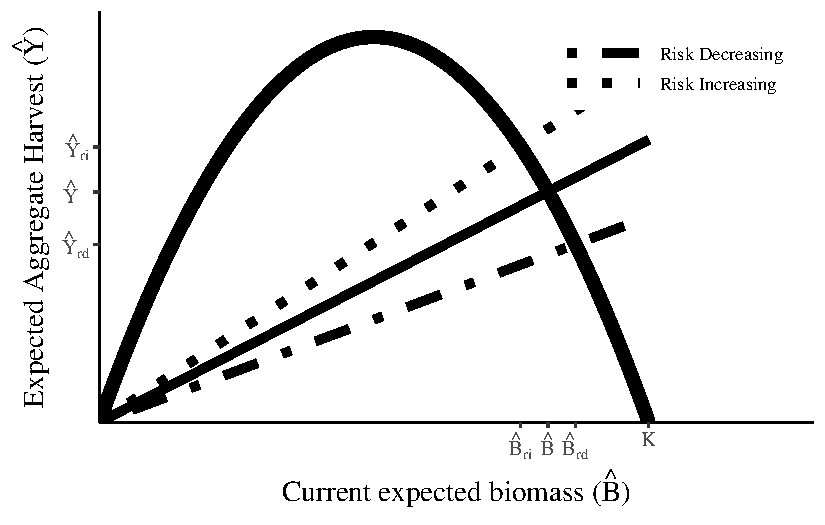
\includegraphics{ibi-behavior_files/figure-pdf/fig-synas-1.pdf}

}

\caption{\label{fig-synas}Expected steady state biomass and aggregate
harvest levels change with index insurance in common-pool fisheries. An
initial pre-insurance equilibrium exists at the intersection of the
growth curve and mean linear production (solid line). If the underlying
inputs are risk increasing the curve shifts to the left (dotted line)
with index insurance. If the underlying inputs are risk decreasing the
curve shifts to the right (dot-dash line) with index insurance.}

\end{figure}

Risk effects determine the impact index insurance has on fishery
conservation even in competitive common-pool extraction. However, risk
effects remain an elusive concept in fisheries. It is unclear how to
preemptively identify fishery risk effects. To date, only one study has
quantified risk effects in a fishery. Asche \emph{et al.} (2020) used
data from four Norwegian fishing fleets to measure three input responses
to risk. Each fishery possessed unique mixes of both risk increasing and
decreasing inputs. For example, labor was found to be a risk decreasing
input across all four groups. Capital was risk increasing for coastal
seiners and trawlers, but was risk decreasing for purse seiners and
trawlers. Fuel had a lower, but statistically significant positive risk
increasing measure for three of the four industry groups.

Single variable aggregate effort measures are useful in
surplus-production models, but do not reflect the complexity of fisher
decisions. As Asche \emph{et al.} (2020) demonstrates, fishers often use
multiple inputs to harvest fish. Index insurance may raise or lower
individual inputs depending on their own unique risk effects, but the
overall direction of harvest decisions may not be so clear. Interactions
between the inputs could override effects of index insurance on
individual inputs. Little research has been done on multiple input
insurance models. Ramaswami (1993) only examined the total production
variance impacts on total harvest changes with insurance, but does not
elaborate on the response of specific inputs. The next section explores
how multiple inputs interact with each other and insurance to provide a
a more comprehensive picture of how index insurance will impact
fisheries.

\hypertarget{sec-multi}{%
\section{Insurance with multiple inputs}\label{sec-multi}}

We simplify the general model in Equation~\ref{eq-max} by using two
inputs, \(X\in\{{x_a,x_b}\}\) to better understand the impact of
insurance on multiple fishery inputs. Adding more variables complicates
the model without adding any additional insights. The complexities of
input interactions sufficiently arise with two inputs to demonstrate our
intended purpose.

The original specification of Just and Pope make no assumption on the
form of the second derivative of the risk effect function. We postulate
reasonable assumptions on the risk effects function to assist with
comparative statics later on. The marginal impact of adding an input to
production variance should have diminishing effects, because it is
impossible to completely eliminate risk or experience infinite risks.
Therefore, when \(h_{x_a}(X^i)>0 \rightarrow h_{x_ax_a}(X^i)<0\), and
when \(h_{x_a}(X^i)<0 \rightarrow h_{x_ax_a}(X^i)>0\). The cross partial
of risk effects on production
\(\frac{\partial h}{\partial x_a \partial x_b}\) must also be flexible
and depend on how inputs interact with each other. For example, if
adding an input does not contribute to the marginal risk effect of
another input then \(\frac{\partial h}{\partial x_a \partial x_b}=0\).
Inputs interactions could be complementary in that adding a risk
decreasing input further enhances the risk reducing properties of the
other inputs, \(\frac{\partial h}{\partial x_a \partial x_b}>0\). In
other instances the inputs may interact counter actively in that adding
more of a risk increasing input might reduce the effect of a risk
decreasing input, \(\frac{\partial h^i}{\partial x_a \partial x_b}<0\).
In principle, when inputs share the same direction of risk effects,
their cross partial ought to be complementary, and when inputs have
opposite risk effects they will be counter productive.

We use the same insurance design from the previous section where
payouts, \(\gamma\), are triggered by \(\omega<0\), and we can partition
profit into good states and bad states. Fishers now maximize expected
utility by selecting two inputs.

\begin{equation}\protect\hypertarget{eq-max2}{}{
\begin{aligned}
U\equiv\max_{x_a^i,x_b^i}\mathbb{E}[U]&=F(\bar\omega)\mathbb{E}[u(\pi^i(X^i,\hat{B}(X^i,Y(X^{\sim j})),\omega)+(1-F(\bar\omega))\gamma)|\omega <\bar\omega]\\
&+(1-F(\bar\omega))\mathbb{E}[u(\pi^i(X^i,\hat{B}(X^i,Y(X^{\sim j})),\omega)-F(\hat\omega)\gamma)|\omega>\bar\omega]
\end{aligned}
}\label{eq-max2}\end{equation}

Taking the first order conditions yields:

\begin{equation}\protect\hypertarget{eq-foc1}{}{
\begin{aligned}
\frac{\partial U}{\partial x_a^i}=&F(\bar\omega)\mathbb{E}[u_{x_a}(\pi^i(X^i,\hat{B}(X^i,Y(X^{\sim j})),\omega)+(1-F(\bar\omega))\gamma)|\omega <\bar\omega]\frac{\partial \mathbb{E}[\pi^i|\omega<\bar\omega]}{\partial x^i_a}\\
&+(1-F(\bar\omega))\mathbb{E}[u_{x_a}(\pi^i(X^i,\hat{B}(X^i,Y(X^{\sim j})),\omega)+-F(\bar\omega)\gamma)|\omega >\bar\omega]\frac{\partial \mathbb{E}[\pi^i|\omega>\bar\omega]}{\partial x^i_a}\\
\frac{\partial U}{\partial x^i_b}=&F(\bar\omega)\mathbb{E}[u_{x_b}(\pi^i(X^i,\hat{B}(X^i,Y(X^{\sim j})),\omega)+(1-F(\bar\omega))\gamma)|\omega <\bar\omega]\frac{\partial \mathbb{E}[\pi^i|\omega<\bar\omega]}{\partial x^i_b} \\
&+(1-F(\bar\omega))\mathbb{E}[u_{x_b}(\pi^i(X^i,\hat{B}(X^i,Y(X^{\sim j})),\omega)+-F(\bar\omega)\gamma)|\omega >\bar\omega]\frac{\partial \mathbb{E}[\pi^i|\omega>\bar\omega]}{\partial x^i_b}\\
\end{aligned}
}\label{eq-foc1}\end{equation}

Given the first order condition is satisfied, we can use the implicit
function theorem (IFT) to look at the impact of a change in the
exogenous insurance contract locally at the input solutions. Applying
IFT and Cramer's Rule yields a system of equations that determine the
impact of insurance on each optimal input:

\begin{equation}\protect\hypertarget{eq-ivtsol}{}{
\begin{aligned}
&\frac{\partial x^i_a}{\partial \gamma}=\frac{-1}{Det}\left[\frac{\partial U}{\partial x^i_b \partial x^i_b}\frac{\partial U}{\partial x^i_a \partial \gamma}-\frac{\partial U}{\partial x^i_a \partial x^i_b}\frac{\partial U}{\partial x^i_b \partial \gamma}\right] \\
&\frac{\partial x^i_b}{\partial \gamma}=\frac{-1}{Det}\left[\frac{-\partial U}{\partial x^i_b \partial x^i_a}\frac{\partial U}{\partial x^i_a \partial \gamma}+\frac{\partial U}{\partial x^i_a \partial x^i_a}\frac{\partial U}{\partial x^i_b \partial \gamma}\right]
\end{aligned}
}\label{eq-ivtsol}\end{equation}

Because the determinate will always be positive by the definition of the
second order condition, we can focus on the interior of the brackets. If
positive, then insurance will lower use of that specific input and vice
versa if negative. The partial derivatives are necessary to sign
Equation~\ref{eq-ivtsol}. Their complete derivations are included in the
appendix. The complex interaction between the partial effects of inputs
and insurance presents a challenge to understanding the impacts of index
insurance on fisheries. Specific conditions must be met to determine the
overall impact of index insurance on inputs, otherwise the effect could
go either way despite the risk increasing or decreasing characteristic
of an individual input.

\begin{proposition}[]\protect\hypertarget{prp-samre}{}\label{prp-samre}

In common-pool fisheries with multiple inputs, index insurance will
change the optimal use of a specific input in accordance to an input's
own risk effect when the following sufficient condition is true:

\(\frac{\partial U}{\partial x^i_a\partial x^i_b}>0\) when both inputs
share the same risk effects, and
\(\frac{\partial U}{\partial x^i_a\partial x^i_b}<0\) when inputs have
opposite risk effects.

Otherwise, Index Insurance will have ambiguous effects on optimal input
choice.

\end{proposition}

\begin{proof}

Corollary~\ref{cor-mp} allows us to sign the partial equations
\(\frac{\partial U}{\partial x^i_a\partial \gamma}\) and
\(\frac{\partial U}{\partial x^i_b\partial \gamma}\)
(Equation~\ref{eq-kgam} and Equation~\ref{eq-lgam} in the appendix) for
any risk effect on either input. Concave utility by definition leads to
\(u_{xx}<0\). For simplicity, we will only focus on
\(\frac{\partial U}{\partial x^i_a\partial \gamma}\), but all applies
equally to \(\frac{\partial U}{\partial x^i_b\partial \gamma}\).
Insurance payouts equalize profits between different states. If
insurance completely covers all loss and \(x^i_a\) is risk increasing,
then \(\frac{\partial U}{\partial x_a\partial \gamma}\) is positive.

\begin{equation}\protect\hypertarget{eq-kgamsol}{}{
\frac{\partial U}{\partial x_a \partial \gamma}=\overbrace{\overbrace{(1-F(\bar\omega))u_{x_ax_a}(\cdot)}^{-}\overbrace{[\frac{\partial \mathbb{E}[\pi^i|w<\bar\omega]}{\partial x_a}-\frac{\partial \mathbb{E}[\pi^i|w>\bar\omega]}{\partial x_a}]}^{-}}^{+}
}\label{eq-kgamsol}\end{equation}

Suppose both inputs are risk increasing so
\(\frac{\partial U}{\partial x^i_a\partial \gamma}\) and
\(\frac{\partial U}{\partial x^i_b\partial \gamma}\) are positive. The
only way for Equation~\ref{eq-ivtsol} to be unambiguously positive is
for \(\frac{\partial U}{\partial x^i_a\partial x^i_b}\) and
\(\frac{\partial U}{\partial x^i_a\partial x^i_b}\)
(Equation~\ref{eq-crossl} and Equation~\ref{eq-crossk} in the appendix)
to be positive.

\[
\begin{aligned}
&\frac{\partial x^i_a}{\partial \gamma}=\overbrace{\frac{-1}{Det}}^{-}\left[\overbrace{\overbrace{\frac{\partial U}{\partial x^i_b \partial x^i_b}}^{-}\overbrace{\frac{\partial U}{\partial x^i_a \partial \gamma}}^{+}\overbrace{-\frac{\partial U}{\partial x^i_a \partial x^i_b}}^{-}\overbrace{\frac{\partial U}{\partial x^i_a \partial \gamma}}^{+}}^{-}\right] >0\\
&\frac{\partial x^i_b}{\partial \gamma}=\overbrace{\frac{-1}{Det}}^{-}\left[\overbrace{\overbrace{\frac{-\partial U}{\partial x^i_b \partial x^i_a}}^{-}\overbrace{\frac{\partial U}{\partial x^i_a \partial \gamma}}^{+}+\overbrace{\frac{\partial U}{\partial x^i_a \partial x^i_a}}^{-}\overbrace{\frac{\partial U}{\partial x^i_b \partial \gamma}}^{+}}^{-}\right]>0
\end{aligned}
\]

Both risk increasing inputs will be raised with index insurance.
Repeating the same steps above with risk decreasing inputs shows both
inputs unambiguously decrease with index insurance.

Now suppose inputs have mixed risk effects. For simplicity, \(x^i_a\)
will be risk increasing and \(x^i_b\) will be risk decreasing. The
results will hold for the opposite case. By Corollary~\ref{cor-mp},
\(\frac{\partial U}{\partial x^i_a\partial \gamma}\) is positive, while
\(\frac{\partial U}{\partial x^i_b\partial \gamma}\) is negative.
Equation~\ref{eq-ivtsol} will be unambiguously positive if
\(\frac{\partial U}{\partial x^i_a\partial x^i_b}\) and
\(\frac{\partial U}{\partial x^i_b\partial x^i_a}\) are negative.

\[
\begin{aligned}
&\frac{\partial x^i_a}{\partial \gamma}=\overbrace{\frac{-1}{Det}}^{-}\left[\overbrace{\overbrace{\frac{\partial U}{\partial x^i_b\partial x^i_b}}^{-}\overbrace{\frac{\partial U}{\partial x^i_a \partial \gamma}}^{+}\overbrace{-\frac{\partial U}{\partial x^i_a \partial x^i_b}}^{+}\overbrace{\frac{\partial U}{\partial x^i_b\partial \gamma}}^{-}}^{-}\right] >0\\
&\frac{\partial x^i_b}{\partial \gamma}=\overbrace{\frac{-1}{Det}}^{-}\left[\overbrace{\overbrace{\frac{-\partial U}{\partial x^i_b\partial x^i_a}}^{+}\overbrace{\frac{\partial U}{\partial x^i_a \partial \gamma}}^{+}+\overbrace{\frac{\partial U}{\partial x^i_a \partial x^i_a}}^{-}\overbrace{\frac{\partial U}{\partial x^i_b\partial \gamma}}^{-}}^{+}\right]<0
\end{aligned}
\]

The risk increasing input will be raised with index insurance, while the
risk decreasing input will be lowered.

If these conditions do not hold, then it is impossible to determine
which additive element outweighs the other, and the insurance effects on
optimal input use will be ambiguous regardless of the underlying risk
effects of an input.

\end{proof}

Proposition~\ref{prp-samre} shows that index insurance can have clear
impacts on input use even in complex settings with multiple inputs
provided the sufficient condition holds. However, it is not clear
ex-ante what the sign of the cross partial inputs of the first order
condition should be. \(\frac{\partial U}{\partial x^i_a\partial x^i_b}\)
and \(\frac{\partial U}{\partial x^i_b\partial x^i_a}\) themselves could
be ambiguous. As shown in the appendix, rearranging
\(\frac{\partial U}{\partial x^i_a\partial x^i_b}\) and
\(\frac{\partial U}{\partial x^i_b\partial x^i_a}\) shows the relative
weight between the marginal profits of each input and the risk effects
cross partial influence the overall sign of first order cross partials.
Essentially, fishers change their inputs depending on whether a given
input makes the other input more productive than the risk it adds.
Whether inputs are complementary or counteractive in their risk effects
influence the sign of the cross partial. When inputs share risk effects,
they ought to increase the risk effects of each other. Therefore the
cross partial is more likely to be negative when inputs share risk
effects and positive when they are complementary following the
sufficient conditions proposed in Proposition~\ref{prp-samre}.

Even with two inputs, ambiguity on the optimal use exists. Extending to
more inputs introduces more interactions among the inputs, and the
relatively weighting between marginal productivity and the risk effect
cross partials is even harder to sign. Ramaswami (1993) used this
complexity as a justification to only examine the total variance of
production with a vector of inputs. Proposition~\ref{prp-samre} helps
elucidate his observations, while providing some understanding of how
different inputs could change when fishers use a variety of inputs.
Specific inputs could have different external environmental and
community impacts. Being better able to predict how index insurance
changes those inputs, and their ensuing impacts on a fishery, will help
minimize any negative impacts that could arise.

Despite the seemingly rigid conditions, Proposition~\ref{prp-samre}
provides useful insight into the behavioral effects insurance will have
when fishers use multiple inputs. It states that when the conditions
hold, the direction all inputs should change is based solely on the
characteristics of their own risk effects. Other inputs may influence
the magnitude of change, but the direction is unequivocal. It remains
unclear what the overall impacts on conservation will be in a multiple
input setting. Differences in mean production elasticity lead to
different magnitudes of change in input use. The overall change in
harvest, and thus conservation, depends on the aggregate change in
harvest. For example, a decline in use for a risk decreasing input
compared to an equivalent increase in use of a risk increasing input may
not lead to lower harvest if the risk increasing input is relatively
more productive.

The next section uses simulations to show the total impact on harvest
can vary substantially, and that the conditions to ensure unambiguous
input change can be met. Though when applied with real world estimates
of risk effects, the conditions may not hold and the effects of index
insurance does not follow simple rules.

\hypertarget{sec-sim}{%
\section{Numerical Simulations}\label{sec-sim}}

We use numerical simulation to test the necessary conditions in
Proposition~\ref{prp-samre} and to determine the magnitude of change in
input use for Norwegian fisheries using the parameters found in Asche
\emph{et al.} (2020). First, we present the simulations from the two
input case to gain additional insight into how index insurance changes
multiple inputs. Fishers earn profit through harvest with a Just and
Pope production function with mean biomass normalized to one, and convex
cost function. Inputs \(X \in \{x_a,x_b\}\) are replaced with capital
(\(k\)) and labor (\(l\)) to ground the interpretation of results in
inputs practically used by fishers.

\begin{equation}\protect\hypertarget{eq-sim}{}{
\pi(k,l)=\hat{B}k^{\alpha_k}l^{\alpha_l}+\omega k^{\beta_k}l^{\beta_l}-c_kk^2-c_ll^2
}\label{eq-sim}\end{equation}

Random shocks (\(\omega\)) are distributed normally with a mean of zero
and a standard deviation of \(\sigma_w\). Capital (\(k\)) and labor
(\(l\)) have both mean production elasticities (\(\alpha_k\) and
\(\alpha_l\)) and flexible risk elasticities (\(\beta_k\) and
\(\beta_l\)). Fishers choose both capital and labor to maximize expected
utility with constant absolute risk aversion (CARA).

Multiple index insurance policies are tested through changes in coverage
and trigger levels. One scenario sets an exogenous constant payout
amounts between 0-200\% of pre-insurance profit, and the other allows
fishers to endogenously choose payouts. The theoretical results of
Section~\ref{sec-common} and Section~\ref{sec-multi} provide comparative
statics on \(\gamma\) payouts as a means to test whether some insurance
is preferred to no insurance and how input use would change. Since the
sign remains the same for any \(\gamma\), the endogenous choice will
also maintain the same sign. However, the magnitudes of input use change
will depend on the level of \(\gamma\). Allowing fishers to choose
insurance coverage ensures that the choice of insurance and input use
changes are welfare improving and will not bias input choices with over
or under investment of insurance.

Trigger levels are set to engage at any below average weather or for
shocks of more than 75\% loss. All premiums are actuarilly fair. Risk
effects vary between -0.7 and 0.7 with iterative increases of 0.1
ignoring situations of 0 risk effects. Fishers can posses low, medium,
and high mean production elasticity values
\(\alpha\in\{0.25,0.5,0.75\}\). Coefficient of constant absolute risk
aversion ranges from 1 to 3. Within each scenario, a Monte Carlo
simulation creates 1000 weather random weather shocks with three
variants of standard deviation \(\sigma_w\in\{0.33,0.5,1\}\).

\hypertarget{sec-simres}{%
\subsection{Numerical simulation results}\label{sec-simres}}

Increasing insurance incentivizes fishers to use more risk decreasing
inputs and less risk increasing inputs (Figure~\ref{fig-ins}). These
results confirm Proposition~\ref{prp-samre}, and show the conditions of
Proposition~\ref{prp-samre} can be satisfied with CARA utility and a
Just-Pope Production function (Figure~\ref{fig-ins}). The direction of
input use is also stable as each class of input is monotonically
increasing or decreasing with more insurance coverage. Inputs follow
expected changes in use given their own risk effect even when risk
effects are mixed. Capital is risk decreasing in the bottom left panel
and decreases with more insurance while the risk increasing labor
increases. The opposite trend occurs in the top right panel.

Index insurance also increases utility shown by the green lines in
Figure~\ref{fig-ins}, but there exists an optimal amount of insurance
coverage for fishers. The optimal values of insurance are generally
lower when fishers use risk decreasing inputs. Notice the peak of the
green line in the bottom right quadrant of Figure~\ref{fig-ins} is
closer to 0 than that of the top left quadrant. Even in the mixed case,
the optimal amount of coverage is lower than when both inputs are risk
increasing. Risk decreasing inputs and insurance act as substitutes for
each other as they both lower fisher income variance. Risk decreasing
inputs still contribute to production while simultaneously reducing
variance. Insurance lowers the need of risk decreasing inputs for their
risk reduction qualities, but cannot fully compensate for the foregone
production. Thus, fishers will choose to use insurance until the
opportunity cost of lost marginal production is equal to insurance gains
in marginal risk protection.

Fishers are more willing to use risk increasing inputs with insurance
because the insurance protects from the added risk of more inputs.
Purchasing more insurance provides greater protection creating a
feedback loop that greatly expands productive input use.

\begin{figure}

{\centering 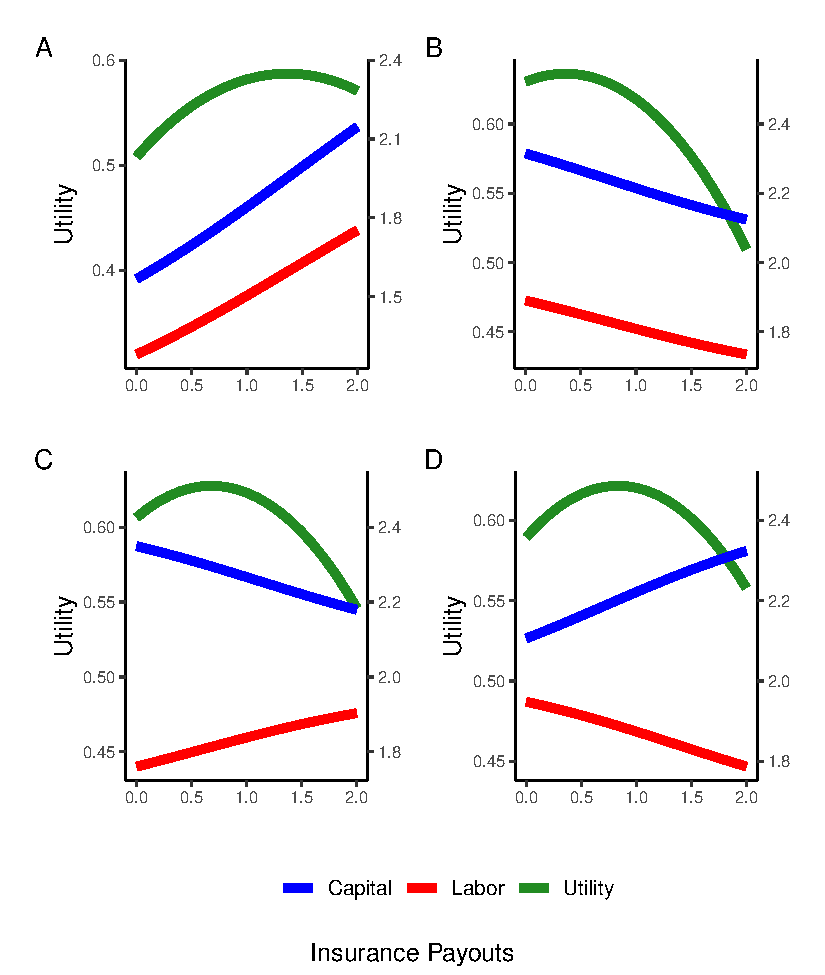
\includegraphics{ibi-behavior_files/figure-pdf/fig-ins-1.pdf}

}

\caption{\label{fig-ins}Fishers choose capital (blue line) and labor
(red line) to maximize utility (green line) for given insurance
contracts that offer more coverage along the x-axis. Fisher utility is
concave in all insurance payouts with CARA utility.}

\end{figure}

Figure~\ref{fig-ins} shows that conditions of
Proposition~\ref{prp-samre} can be satisfied, but it does not show the
conservation outcomes of index insurance. Fishers use the new choice of
inputs to change their overall harvest and thus impact on the biomass of
fish stocks. Harvest changes are influenced by the relative combination
of risk effects, mean production elastiticies, and the amount of
insurance (Figure~\ref{fig-multi-h-even}). Fishers reduce harvest more
aggressively with risk decreasing inputs when offered a set contract of
50\% coverage of pre-insurance profits (Panel A) relative to their
optimal insurance choice (Panel B). Allowing fishers to choose their
insurance coverage leads them to increase harvest more with risk
increasing inputs. A 50\% coverage is an overinvestment in insurance for
risk decreasing inputs and an underinvestment for risk increasing
inputs.

Mixed risk effects have more nuance in overall harvest as seen in the
top left and bottom right quadrants of each panel in
Figure~\ref{fig-multi-h-even}. Risk increasing inputs appear to dominant
risk reducing inputs leading to generally more increases in harvest. For
example, when an input has a risk increasing effect of 0.5, harvest
still increases even if the other input has a stronger risk reducing
effect at -0.7. The reduction in the risk decreasing output can outweigh
the increase in the risk increasing input if the risk decreasing effect
is much stronger than the risk increasing effect. For all risk effects
at -0.7, when the other input has a risk effect \textless0.3, harvest
decreases. In all cases, the change in harvest is quite small ranging
from 0.8\%-5\%.

\begin{figure}

{\centering 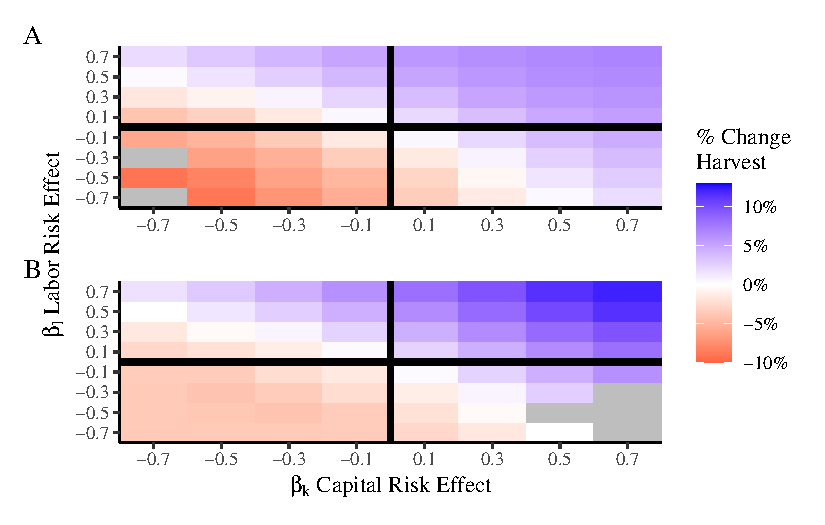
\includegraphics{ibi-behavior_files/figure-pdf/fig-multi-h-even-1.pdf}

}

\caption{\label{fig-multi-h-even}Percent change in fishing harvest when
fishers use index insurance with low mean elasticity values
(\(\alpha_{k,l}=0.25\)). In Panel A, Insurance payouts are a set
variable. In Panel B, fishers choose insurance payouts. Red colors show
overall decreases in harvest while blue colors show overall increases in
harvest. Grey boxes indicate simulations where it was not profitable to
fish at all with the given production inputs.}

\end{figure}

Increasing the mean elasticities exacerbates the discrepancies between
changes in harvest through index insurance
(Figure~\ref{fig-multi-h-even-hi}). When the productivity of harvest
(\(\alpha\)) is higher, the tradeoff between reducing variance and catch
changes. When the mean production elasticity is increased to 0.5, the
maximum amount of observed harvest is 45\% when fishers choose their
insurance levels while the greatest reduction is only 8\%. Higher mean
elasticities imply a greater change in harvest and profit with changes
in an input. Lowering use will have a proportionally greater tradeoff
between risk protection and income for risk decreasing inputs at higher
mean production elasticities.

\begin{figure}

{\centering 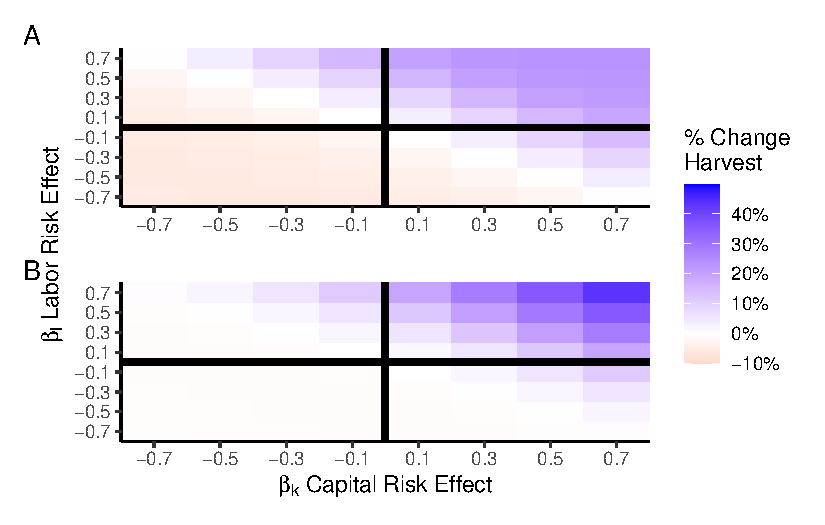
\includegraphics{ibi-behavior_files/figure-pdf/fig-multi-h-even-hi-1.pdf}

}

\caption{\label{fig-multi-h-even-hi}When fishers choose insurnace, they
drastically increase (blue) harvest with risk increasing relative to no
insurance harvest. Inputs share the same mean elasticity
(\(\alpha_{k,l}=0.5\)). Insurance payouts are exogenously set at 50\%
profits in Panel A. Insurance payouts are chosen in Panel B. Risk
aversion is set to 1. Weather variance is 0.5. Below the dotted line
show cases where harvest was reduced.}

\end{figure}

The magnitude of input use also changes based on the fisher risk
preferences, weather risk, and contract terms. We extract simulation
results where both inputs have the same risk effects and both have mean
production elasticities of 0.5 (\(\alpha_k=\alpha_l=0.5\)) to more
clearly isolate these effects (Figure~\ref{fig-multi-para}). More risk
averse fishers respond more aggressively to insurance and make
relatively more changes toward their input decisions (Panel A in
Figure~\ref{fig-multi-para}). Risk aversion implies more sensitivity
towards risk. The protection from insurance has greater marginal value
for more risk averse fishers. Greater marginal value of insurance means
they can invest less into risk reducing inputs than before, and have
more protection from greater shocks with risk increasing inputs.

Fisher input choice are much more responsive to insurance protection
from larger environmental risks (Panel B Figure~\ref{fig-multi-para}).
Similar to risk aversion, the greater the shocks the greater the
marginal value of insurance is to mitigate those shocks. In more
volatile environments, insurance provides significantly more income
smoothing leading to similar incentives as the higher risk aversion
example.

Trigger levels also influence fisher behavior in interesting ways. When
insurance covers more catastrophic events, such as shocks that are in
the 75th percentile, fishers respond more aggressively if they are using
risk decreasing inputs compared to risk increasing inputs (Panel C
Figure~\ref{fig-multi-para}). Payouts occur in disastrous events at
higher levels of coverage. When these larger shocks occur adding more
risk increasing inputs could lead to more catastrophic outcomes. The
incentive to increase input use is reduced in this case. Risk decreasing
inputs on the other hand are more easily substitutable with insurance
when greater shocks occur. Hence, the incentive for fishers to reduce
input use is greater.

\begin{figure}

{\centering 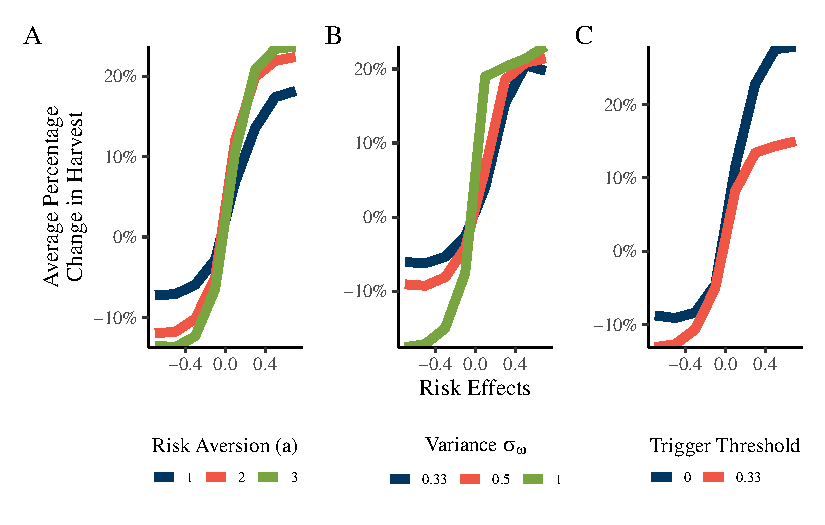
\includegraphics{ibi-behavior_files/figure-pdf/fig-multi-para-1.pdf}

}

\caption{\label{fig-multi-para}Risk Aversion (A), trigger level (B), and
weather variance (C) all influence the magnitude of change in harvest.
Mean production elasticity is 0.5 for both inputs. Average percent
change in harvest (y-axis) is summarized across all other parameter
combinations for each risk effect combination (x-axis) that are the same
for both inputs (e.g.~\(-0.4=\beta_k=\beta_l\))}

\end{figure}

\hypertarget{application-to-real-world-fisheries}{%
\subsection{Application to Real World
Fisheries}\label{application-to-real-world-fisheries}}

Asche et al., (2020) aggregated by vessel type and not species, so there
is no reasonable estimate for biomass. They accounted for biomass using
fixed effects in their regression, but without additional information,
our simulations normalize biomass to 1 and only focus on the relative
change in inputs and aggregate harvest. The simulation model extends the
two input case to include fuel (\(f\)).

\begin{equation}\protect\hypertarget{eq-sim3}{}{
\pi(k,l,f)=k^{\alpha_k}l^{\alpha_l}f^{\alpha_f}+\omega k^{\beta_k}l^{\beta_l}k^{\beta_f}-c_kk^2-c_ll^2-c_ff^2
}\label{eq-sim3}\end{equation}

Fishers in the simulation choose inputs and insurance coverage to
maximize expected utility. The endogenous choice is necessary to ensure
fishers choose welfare improving amounts. Ex-ante it is unclear what the
amount of insurance should be. Also the simulation results from
Section~\ref{sec-simres} indicate that over investing in insurance will
lead to relatively greater reductions in risk reducing inputs, which
would introduce bias in this application.

\begin{equation}\protect\hypertarget{eq-maxasche}{}{
\begin{aligned}
U&\equiv\max_{\gamma,k,l,f}\mathbb{E}[u]=\mathbb{E}[u(k^{\alpha_k}l^{\alpha_l}f^{\alpha_f}+\omega k^{\beta_k}l^{\beta_l}k^{\beta_f}-c_kk^2-c_ll^2-c_ff^2+\mathbb{I}(\gamma)]\\
\mathbb{I}(\gamma)&=\begin{cases}-\rho\gamma & \text{if } \omega\ge \bar\omega\\
(1-\rho)\gamma & \text{if } \omega<\bar\omega
\end{cases}
\end{aligned}
}\label{eq-maxasche}\end{equation}

Table~\ref{tbl-asche} shows the production and risk elasticities of the
four vessel types used in the simulation. While not all elasticities
were found to be statistically different from zero, we used their raw
values because dropping only those variables that are significant in
both matching parameters would have kept only a few valid combinations.
All non-significant elasticities led to small changes as expected, but
their interactions with other inputs could partially drive some of the
observed outcomes.

\hypertarget{tbl-asche}{}
\begin{longtable}[]{@{}
  >{\raggedright\arraybackslash}p{(\columnwidth - 12\tabcolsep) * \real{0.2410}}
  >{\raggedleft\arraybackslash}p{(\columnwidth - 12\tabcolsep) * \real{0.1325}}
  >{\raggedleft\arraybackslash}p{(\columnwidth - 12\tabcolsep) * \real{0.1325}}
  >{\raggedleft\arraybackslash}p{(\columnwidth - 12\tabcolsep) * \real{0.1325}}
  >{\raggedleft\arraybackslash}p{(\columnwidth - 12\tabcolsep) * \real{0.1205}}
  >{\raggedleft\arraybackslash}p{(\columnwidth - 12\tabcolsep) * \real{0.1205}}
  >{\raggedleft\arraybackslash}p{(\columnwidth - 12\tabcolsep) * \real{0.1205}}@{}}
\caption{\label{tbl-asche}Production and Risk elasticities of Norwegian
Fisheries from Asche et al., (2020)}\tabularnewline
\toprule\noalign{}
\begin{minipage}[b]{\linewidth}\raggedright
\end{minipage} & \begin{minipage}[b]{\linewidth}\raggedleft
\(\alpha_k\)
\end{minipage} & \begin{minipage}[b]{\linewidth}\raggedleft
\(\alpha_l\)
\end{minipage} & \begin{minipage}[b]{\linewidth}\raggedleft
\(\alpha_f\)
\end{minipage} & \begin{minipage}[b]{\linewidth}\raggedleft
\(\beta_k\)
\end{minipage} & \begin{minipage}[b]{\linewidth}\raggedleft
\(\beta_l\)
\end{minipage} & \begin{minipage}[b]{\linewidth}\raggedleft
\(\beta_f\)
\end{minipage} \\
\midrule\noalign{}
\endfirsthead
\toprule\noalign{}
\begin{minipage}[b]{\linewidth}\raggedright
\end{minipage} & \begin{minipage}[b]{\linewidth}\raggedleft
\(\alpha_k\)
\end{minipage} & \begin{minipage}[b]{\linewidth}\raggedleft
\(\alpha_l\)
\end{minipage} & \begin{minipage}[b]{\linewidth}\raggedleft
\(\alpha_f\)
\end{minipage} & \begin{minipage}[b]{\linewidth}\raggedleft
\(\beta_k\)
\end{minipage} & \begin{minipage}[b]{\linewidth}\raggedleft
\(\beta_l\)
\end{minipage} & \begin{minipage}[b]{\linewidth}\raggedleft
\(\beta_f\)
\end{minipage} \\
\midrule\noalign{}
\endhead
\bottomrule\noalign{}
\endlastfoot
Coastal Seiners & 0.294 & 0.421 & 0.457 & 0.184 & -0.432 & 0.119 \\
Coastal Groundfish & 0.463 & 0.421 & 0.355 & 0.965 & -0.080 & 0.113 \\
Purse Seiners & 0.941 & -0.108 & 0.605 & -0.454 & -0.231 & 0.160 \\
Groundfish Trawlers & 0.210 & 0.106 & 0.531 & -2.788 & -0.110 &
-0.024 \\
\end{longtable}

Applying index insurance in Norwegian fisheries will lead to changes in
input use and overall harvest. Table~\ref{tbl-nor} shows that index
insurance would have lead to a maximum change of 15\% in total harvest
for the coastal groundfish fishery. This was primarily driven by large
increases in capital (20.36\%) and fuel (8.89\%). All inputs had
relatively similar mean production elasticities, but capital was
strongly risk increasing with the highest positive risk elasticity.
Labor was a risk decreasing input, but also rose with insurance. This is
an example where the conditions of Proposition~\ref{prp-samre} do not
hold. The large discrepancy in production risk elastiticites is probably
a reason for this in addition to the interactions terms at play by
adding a third input. The chosen insurance payout was also much higher
than the other vessel types. This reflects the observation from
Figure~\ref{fig-ins} that that fishers choose higher levels of insurance
coverage as a means to substitute the additional risk they are taking
with expanded production.

Purse seiners saw the largest reduction in overall harvest. Capital for
purse seiners is the most productive input out of all fisheries and
inputs. Because it is risk reducing, it dominates the slightly risk
increasing fuel input to lead the entire fishery to reduce harvest by
6.3\%. this shows another case where the conditions of
Proposition~\ref{prp-samre} do not hold. Despite being a risk increasing
input, fuel use declined with index insurance. Labor allocations did not
change. No labor was allocated in either optimal choice, because the
production elasticity was negative. Insurance payouts were also higher
than the other fisheries that saw reductions. The high productivity of
capital and fuel were most likely driving this result because small
reductions in these productive inputs needed larger compensations.

Coastal seiners show the conditions for Proposition~\ref{prp-samre} can
hold in the real world with multiple inputs. All input use changes
followed their respective risk effects. Capital (0.44\%) and fuel
(0.11\%) both increased, while labor (-1.01\%) decreased. In aggregate,
there was a small reduction in harvest (-0.3\%). While insurance led to
a change, it was rather small and would not have a large impact on the
fishery. The counteractive effects of the risk effects may negate some
of the desire to change production as insurance incentivizes both
increases and decreases in harvest.

Inputs in the groundfish trawler industry were all risk reducing.
Unsurprisingly, each input saw a reduction in use when index insurance
was offered. Capital was extremely risk reducing and saw a 4.14\%
reduction in use, but was a relatively less productive input so overall
harvest changed by only 1.4\%. Optimal insurance payouts were the lowest
in this fishery reflecting the substitution of insurance and risk
reducing inputs.

\hypertarget{tbl-nor}{}
\begin{longtable}[]{@{}
  >{\raggedright\arraybackslash}p{(\columnwidth - 10\tabcolsep) * \real{0.2597}}
  >{\raggedright\arraybackslash}p{(\columnwidth - 10\tabcolsep) * \real{0.1039}}
  >{\raggedright\arraybackslash}p{(\columnwidth - 10\tabcolsep) * \real{0.1039}}
  >{\raggedright\arraybackslash}p{(\columnwidth - 10\tabcolsep) * \real{0.0909}}
  >{\raggedright\arraybackslash}p{(\columnwidth - 10\tabcolsep) * \real{0.1039}}
  >{\raggedleft\arraybackslash}p{(\columnwidth - 10\tabcolsep) * \real{0.3377}}@{}}
\caption{\label{tbl-nor}Percent change in input use and harvest for four
Norwegian fisheries due to index insurance induced moral
hazards.}\tabularnewline
\toprule\noalign{}
\begin{minipage}[b]{\linewidth}\raggedright
\end{minipage} & \begin{minipage}[b]{\linewidth}\raggedright
Capital
\end{minipage} & \begin{minipage}[b]{\linewidth}\raggedright
Labor
\end{minipage} & \begin{minipage}[b]{\linewidth}\raggedright
Fuel
\end{minipage} & \begin{minipage}[b]{\linewidth}\raggedright
Harvest
\end{minipage} & \begin{minipage}[b]{\linewidth}\raggedleft
Insurance Payout \(\gamma\)
\end{minipage} \\
\midrule\noalign{}
\endfirsthead
\toprule\noalign{}
\begin{minipage}[b]{\linewidth}\raggedright
\end{minipage} & \begin{minipage}[b]{\linewidth}\raggedright
Capital
\end{minipage} & \begin{minipage}[b]{\linewidth}\raggedright
Labor
\end{minipage} & \begin{minipage}[b]{\linewidth}\raggedright
Fuel
\end{minipage} & \begin{minipage}[b]{\linewidth}\raggedright
Harvest
\end{minipage} & \begin{minipage}[b]{\linewidth}\raggedleft
Insurance Payout \(\gamma\)
\end{minipage} \\
\midrule\noalign{}
\endhead
\bottomrule\noalign{}
\endlastfoot
Coastal Seiners & 0.44\% & -1.011\% & 0.11\% & -0.3\% & 0.43 \\
Coastal Groundfish & 20.36\% & 6.578\% & 8.89\% & 15.4\% & 1.24 \\
Purse Seiners & -4.39\% & 0.000\% & -3.77\% & -6.3\% & 0.81 \\
Groundfish Trawlers & -4.14\% & -0.979\% & -0.69\% & -1.4\% & 0.23 \\
\end{longtable}

\hypertarget{sec-disc}{%
\section{Discussion}\label{sec-disc}}

Index insurance will have behavioral impacts on fishers' input
decisions, which in turn will lead to changes in fishery sustainability.
The direction and magnitude of impacts are primarily sensitive to the
risk effects of inputs used in production and can have ambiguous
outcomes. We found that traditional fisheries models, such as
Gordon-Schaefer, predict that index insurance will always increase
fishing pressures. These models are inherently risk increasing and do
not adequately capture deeper risk mitigation strategies. Common-pool
resource models using similar structures also contain similar biases.
Bulte and Haagsma (2021) found index insurance will always raise herd
size in common grazing pastures. The underlying production model they
use has risk effects that are always positive like Gordon-Schaefer.
Incorporating more flexible production models that allow for both
positive and negative risk effects presents a more nuanced view of index
insurance.

As shown in this paper, harvest pressures could reduce by 6\% in
Norwegian purse seiners. Norway has well managed fisheries. This would
place these fisheries to the right or near MSY in Figure~\ref{fig-synas}
so that a reduction in 6\% harvest also corresponds to some level of
improved fish stocks. Norwegian coastal groundfish trawlers were
incentivized to increase their harvest by 15.4\% with index insurance.
Without more specific biological information, we cannot extrapolate the
total effect on fish abundance. Whether the changes we estimate for
these Norwegian vessel groups are beneficial or detrimental to the fish
stocks is not clear. Some level of change will occur and need to be
accounted for in the design of index insurance programs. The magnitude
of change indicates while index insurance may not be a conservation
panacea in isolation, it also may not be a destructive tool. The
decision to develop index insurance should revolve around whether it
provides sufficient financial relief for fishing communities when
designed to minimize negative impacts on fish stocks. While not the
focal point of this paper, the average gain in utility from our
simulations was 5\% indicating that index insurance can achieve welfare
improving outcomes for fishers moving forward.

The symmetry of players and the exogenous insurance contract limit
analysis of selection bias and conservation stability. Essentially, our
model assumes that all fishers have access to insurance while making
their decisions and prevents potential free riding. This isolates the
effects of input decisions as everyone has equal responses, but does not
reflect what could happen with fishers with different productivity,
costs, and risk tolerance. All of those elements would inform their
decision on whether to take insurance or not. If fishers are allowed to
individually buy insurance contracts, there could be more risk loving
fishers that choose to take no insurance and gain from less fishing
pressure by the more risk averse insurance takers if inputs are risk
decreasing. The overall change in direction for harvest would be unclear
as it depends on the number and extent of fishers opting out of
insurance.

The direction of index insurance effects on fisher behavior change
hinges on input risk effects. Risk effects need to be reconciled in
fisheries in order to articulate more accurate behavior changes of
fishery index insurance. Crop covers and pesticide provide clear
examples of risk decreasing inputs in agriculture, but what do risk
decreasing inputs look like in fisheries? Asche \emph{et al.} (2020)
provide empirical evidence of the existence of risk decreasing inputs,
but do not elaborate on why or how labor and capital directly decrease
risk. Labor is perhaps the more intuitive risk decreasing input.
Technical expertise of crew and captains can hedge against luck when
fishing (Alvarez \emph{et al.} 2006). Better trained crew can deploy
gear in a safe and timely manner, increasing the likelihood of effective
sets.

Fuel as a risk increasing input in fisheries makes intuitive sense as
well. Fuel is used to power vessels and is a direct cost of fishing. The
more fuel used, the more fishing is occurring. The more fishing that is
occurring, the more risk is being taken on. Every hour at sea increases
the reward, but also the chances of failure.

Capital is a more complex input, because it can be both risk increasing
and decreasing. Capital investments in fisheries typically refer to
vessel tonnage, engine power, and gear technology. The spatiotemporal
dimension of fishing decisions may explain how capital can potentially
possess both risk effects. Fishers have to make decisions on where,
when, and how long to fish that differ from the set grids of agriculture
(Reimer \emph{et al.} 2017). Capital offers protection from risk by
allowing fishers to explore more fishing grounds, use more secure gear,
and fish in more adverse weather conditions. When common pool resources
incentivize the race to fish, having larger vessels may be a risk
reducing input as the sooner a fisher can catch they assure their income
at the expense of other fishers. Adding risk aversion to standard models
of common pool fisheries suggests fishers should lower their capital use
compared to risk neutral allocations (Mesterton-Gibbons 1993; Tilman
\emph{et al.} 2018). Yet, overcapitalization and overfishing are more
often observed in the real world. Either fishers are never risk averse
or the risk effects of capital are not as simple as the standard model
suggests. When capital is allowed to be a risk decreasing, optimal
allocations are much higher than risk neutral equilibrium suggesting
fishers are making rational, risk averse decisions.

Biomass is a crucial fishery input that may also possess risk effects.
To simplify the analysis we focused solely on fisher controlled inputs,
but the stochastic nature of growth in fisheries is a fundamental driver
of risk. Most biological models assume some additive or multiplicative
shock in the growth period. This leads to higher levels of variability
with higher levels of abundance. However, different forms of risk could
be embedded into the biological component of fishery models. Stock
variance could be greater in overfished stocks instead of healthier
ones, reflecting more vulnerability in weaker states (Sims \emph{et al.}
2018). The effects of insurance with these biological risk effects could
lead to unique changes in fisher behavior. Perhaps it strengthens the
trends model in this paper. If insurance protects from more risk,
fishers may be more willing to expose themselves to greater risk at more
vulnerable stock levels. Alternatively, insurance could help mitigate
risk and incentivize fishers to move toward healthier stocks with less
variance by alleviating pressures to fish. Further analysis is required
to understand the full implications of biological risk effects in
fisheries.

The transfer between inputs and insurance reflects the substitution
between self-insurance and formal insurance (Quaas and Baumgärtner
2008). If index insurance is designed to reduce fishing capacity,
efforts must be made to ensure that it does not take away from the self
resiliency of fishers. Labor appears to be consistently risk reducing
and acts as a form of self insurance. If index insurance incentivizes
captains to hire less crew, the stock of fish may be preserved, but less
employment may reverberate throughout the community. Fishing is often a
primary employment opportunity in coastal communities. Lowering
employment options may lead to increased poverty or concentrated wealth.
The resiliency of the community would be compromised rather than
enhanced. The same idea applies to capital. If fishers are over
investing in capital to hedge against some form of risk, policymakers
need to be sure the insurance is replacing maladaptive self insurance
behavior.

The primary form of self insurance in fisheries is management. To this
point our analysis explicitly modeled scenarios without the existence of
management. Most fisheries are managed in some form. The interaction
between management and insurance may be complementary or substitutes.
For example, well managed fisheries that have responsive harvest control
rules may not need insurance. The management system is already providing
the necessary risk protection. Insurance demand and uptake may be low in
these fisheries. Insurance could instead complement management to
provide the financial relief that management cannot offer. Managers
often focus on the biological health of the fishery that can run at odds
with fishers' desires to enhance their income. Insurance can act as the
financial relief and allow managers to pursue more active strategies to
protect fish stocks without political resistance from lowered quotas.
The interaction between insurance and management requires further
investigation especially with the the numerous management strategies
that exist in fisheries.

Design and access of insurance must also consider equity. The current US
federal disaster relief program is inequitable with bias towards large
industrial vessels (Jardine \emph{et al.} 2020). Creating another
program with an equal inequity would be foolhardy. Current US farm
subsidies, including insurance premiums, are heavily skewed towards
large agribusinesses (White and Hoppe 2012). Dimensions of access,
procedural, representation, and distribution must all be built into the
design of new fishery index insurance programs (Fisher \emph{et al.}
2019). For example, small scale fishers may have income constraints that
prevent them from buying the initial contract. Micro-finance options
connected to insurance have been used in agriculture to alleviate this
burden with some success (Dougherty \emph{et al.} 2021). Additionally,
we must ensure that is not only the vessel owners who reap the benefits
of insurance. Deckhands and crew are laid off during closures. If index
insurance payouts are going through the entire fishery, the most
vulnerable to closures must be protected as well. Contract stipulations
could mandate that only cost expenses are covered by payouts thereby
including lost wages to the crew. Agriculture contracts often are
designed to directly cover expenses.

Our model only directly models behavior change through moral hazards.
Index insurance could be designed to incentivize other forms of
sustainable behavior change. We define three pathways insurance can
change behavior: Moral hazards, Quid Pro Quo, and Collective Action.
Moral hazards were proven in this paper to have ambiguous impacts
controlled by the risk characteristics of fishery inputs. Contract
design can shape moral hazards as well. Figure~\ref{fig-multi-para}
Panel C shows that with higher trigger thresholds, fishers are more
incentivized to reduce harvest than increase harvest. Allowing insurees
to choose their triggers has been found to increase insurance uptake
(Lichtenberg and Iglesias (2022)). Well designed contracts can stimulate
demand while guiding more sustainable behavior.

Quid Pro Quo expands contract design to explicitly build in conservation
measures. Fishers would be required to adopt sustainable practices in
order to qualify for insurance. Quid Pro Quo is already used in
agricultural insurance in the form of Good Farm Practices. Farmers must
submit management plans to US Risk Management Agency that clearly
outline their conservation practices in order to qualify for insurance.
Working closely with management agencies, insurance companies could
design contracts that require fishers to follow fishery specific
management practices. For example, fishers may be incentivized to use
more sustainable gear types, have an observer onboard, or reduce
bycatch. Manager input is needed to tailor fishery best practices to
insurance contracts. Further research would need to uncover the full
impact of Quid Pro Quo, but an initial hypothesis would be the fishers
will be willing to adopt sustainable practices so long as the marginal
gain in utility from the insurance is greater or equal to the necessary
sustainable changes. Otherwise fishers will not want to buy the
contracts and the insurance has no binding stipulations to change the
fishery.

Collective action ties insurance premiums to biological outcomes to
leverage the political economy of the fishery. Insures could reduce
premiums in fisheries that have robust management practices such as
adaptive harvest control rules, stock assessments, or marine protected
areas in the vicinity. Fishers could either pressure regulators to adopt
these actions or form industry groups to undertake the required actions.
Insurers would agree to this if triggers are connected to biological
health so that negative shocks are less frequent and thus payouts occur
less. Fishers gain from the insurance premium and the increases
sustainability of harvest with rigorous management in place.

Ultimately, if index insurance is to be used in fisheries, it must be
designed with clear objectives and intentions. Index insurance can meet
objectives of income stability and risk reduction. There has been an
implicit assumption by practitioners that index insurance will always
lead to improved sustainability. Without considering the behavior change
of fishers when adopting insurance, the outcomes may not be as expected.
New insights derived from this paper will help guide the efficient and
sustainable implementation of fisheries index insurance.

\hypertarget{appendix}{%
\section{Appendix}\label{appendix}}

Partial derivatives used to sign Equation~\ref{eq-ivtsol} are shown
below.

\begin{equation}\protect\hypertarget{eq-kk}{}{
\begin{aligned}
\frac{\partial F}{\partial k \partial k}&=(1-p)u''(\pi_g-p\gamma)(\frac{\partial \pi_g}{\partial k})^2+(1-p)u'(\pi_g-p\gamma)\frac{\partial^2 \pi_g}{\partial k\partial k}\\
&+ pu''(\pi_b+(1-p)\gamma)(\frac{\partial \pi_b}{\partial k})^2+pu'(\pi_b+(1-p)\gamma)\frac{\partial^2 \pi_b}{\partial k \partial k}
\end{aligned}
}\label{eq-kk}\end{equation}

\begin{equation}\protect\hypertarget{eq-ll}{}{
\begin{aligned}
\frac{\partial F}{\partial l \partial l}&=(1-p)u''(\pi_g-p\gamma)(\frac{\partial \pi_g}{\partial l})^2+(1-p)u'(\pi_g-p\gamma)\frac{\partial^2 \pi_g}{\partial l\partial l}\\
&+ pu''(\pi_b+(1-p)\gamma)(\frac{\partial \pi_b}{\partial l})^2+pu'(\pi_b+(1-p)\gamma)\frac{\partial^2 \pi_b}{\partial l \partial l}
\end{aligned}
}\label{eq-ll}\end{equation}

\begin{equation}\protect\hypertarget{eq-crossl}{}{
\begin{aligned}
\frac{\partial F}{\partial k \partial l}&=(1-p)u''(\pi_g-p\gamma)\frac{\partial \pi_g}{\partial k}\frac{\partial \pi_g}{\partial l}+(1-p)u'(\pi_g-p\gamma)\frac{\partial \pi_g}{\partial k\partial l}\\
&+ pu''(\pi_b+(1-p)\gamma)\frac{\partial \pi_b}{\partial k}\frac{\partial \pi_b}{\partial l}+pu'(\pi_b+(1-p)\gamma)\frac{\partial \pi_b}{\partial k \partial l}
\end{aligned}
}\label{eq-crossl}\end{equation}

\begin{equation}\protect\hypertarget{eq-crossk}{}{
\begin{aligned}
\frac{\partial F}{\partial l \partial k}&=(1-p)u''(\pi_g-p\gamma)\frac{\partial \pi_g}{\partial l}\frac{\partial \pi_g}{\partial k}+(1-p)u'(\pi_g-p\gamma)\frac{\partial \pi_g}{\partial l\partial k}\\
&+ pu''(\pi_b+(1-p)\gamma)\frac{\partial \pi_b}{\partial l}\frac{\partial \pi_b}{\partial k}+pu'(\pi_b+(1-p)\gamma)\frac{\partial \pi_b}{\partial l \partial k}
\end{aligned}
}\label{eq-crossk}\end{equation}

\begin{equation}\protect\hypertarget{eq-kgam}{}{
\frac{\partial F}{\partial k \partial \gamma}=(1-p)u''(\pi_g-p\gamma)\frac{\partial \pi_g}{\partial k}(-p)+pu''(\pi_b+(1-p)\gamma)\frac{\partial \pi_b}{\partial k}(1-p)
}\label{eq-kgam}\end{equation}

\begin{equation}\protect\hypertarget{eq-lgam}{}{
\frac{\partial F}{\partial l \partial \gamma}=(1-p)u''(\pi_g-p\gamma)\frac{\partial \pi_g}{\partial l}(-p)+pu''(\pi_b+(1-p)\gamma)\frac{\partial \pi_b}{\partial l}(1-p)
}\label{eq-lgam}\end{equation}

Proof of Corollary~\ref{cor-mp}.

\textbf{Corollary 2.1} \emph{Marginal profit in the bad state of the
world is greater (less) than marginal profit in the good state when
\(h_x'(X)<0\) (\(h_x'(X)>0\)). If \(h_x'(X)=0\), the marginal profits
are equivalent in both states.}

By the first order conditions, there exist optimal values of any
individual input \(x_m^{i*}\) that must be chosen before the realization
of the states of the world. Therefore \(h(X^{i*})\), \(f(X^{i*})\), and
\(c(X^{i*})\) are equal across states.

Marginal utility in both states of the world is controlled by risk
effects and the sign of the random variable \(\omega\). Risk increasing
inputs have \(h_x'(X)>0\) by definition. For any input denoted by \(x\)
this holds

\begin{equation}\protect\hypertarget{eq-comppi1}{}{
\begin{aligned}
\frac{\partial \mathbb{E}[\pi^i|\omega<\bar\omega]}{\partial x^{i*}_m}-\frac{\partial \mathbb{E}[\pi^i|\omega>\bar\omega]}{\partial x^{i*}_m}=&\mathbb{E}[\omega h_{x_m^*}(X^{i*})|\omega<\bar\omega]+\cancel{f_{x_m^*}'(X^{i*})\hat{B}(X^{i*},Y(X^{\sim j *}))}+\cancel{f_{x^*_m}(X^{i*})\frac{\partial \hat{B}(X^{i*},Y(X^{\sim j *}))}{\partial x_m^{*}}\frac{\partial Y(X^{\sim j *})}{\partial x^*_m}}-\cancel{c_{x^*_m}(X^{i*})} \\
&\mathbb{E}[\omega h_{x_m^*}(X^{i*})|\omega>\bar\omega]+\cancel{f_{x_m^*}'(X^{i*})\hat{B}(X^{i*},Y(X^{\sim j *}))}+\cancel{f_{x^*_m}(X^{i*})\frac{\partial \hat{B}(X^{i*},Y(X^{\sim j *}))}{\partial x_m^{*}}\frac{\partial Y(X^{\sim j *})}{\partial x^*_m}}-\cancel{c_{x^*_m}(X^{i*})} \\
=&\mathbb{E}[\omega h_{x_m^*}(X^{i*})|\omega<\bar\omega]-\mathbb{E}[\omega h_{x_m^*}(X^{i*})|\omega>\bar\omega]
\end{aligned}
}\label{eq-comppi1}\end{equation}

If an input is risk decreasing then \(h_{x_m}(X^i)<0\). Then
Equation~\ref{eq-comppi1} is positive and marginal profit in the bad
state is greater than the marginal profit in the good state. Adding more
of a risk reducing input reduces the negative impact in the bad state
relative to the good state.

\[
\frac{\partial \mathbb{E}[\pi^i|\omega<\bar\omega]}{\partial x^{i*}_m}-\frac{\partial \mathbb{E}[\pi^i|\omega>\bar\omega]}{\partial x^{i*}_m}=\overbrace{\mathbb{E}[\omega h_{x_m^*}(X^{i*})|\omega<\bar\omega]-\mathbb{E}[\omega h_{x_m^*}(X^{i*})|\omega>\bar\omega]}^{+}
\]

Repeating the same thing for risk increasing inputs \(h_{x_m}(X^i)>0\)
shows that marginal profit in the bad state is less than marginal profit
in the good state.

\[
\frac{\partial \mathbb{E}[\pi^i|\omega<\bar\omega]}{\partial x^{i*}_m}-\frac{\partial \mathbb{E}[\pi^i|\omega>\bar\omega]}{\partial x^{i*}_m}=\overbrace{\mathbb{E}[\omega h_{x_m^*}(X^{i*})|\omega<\bar\omega]-\mathbb{E}[\omega h_{x_m^*}(X^{i*})|\omega>\bar\omega]}^{-}
\]

If inputs have no risk effects then \(h_{x_m}(X^i)=0\). Subbing into
Equation~\ref{eq-comppi1} shows there is no difference in marginal
profits with no risk effects.

\begin{proposition}[]\protect\hypertarget{prp-rn}{}\label{prp-rn}

Risk neutral fishers will not change their input use with index
insurance

\end{proposition}

\begin{proof}

Risk neutrality implies that \(u'(k,l)=0\) and \(u''(k,l)=0\). Subbing
\(u''(k,l)=0\) into both Equation~\ref{eq-kgam} and
Equation~\ref{eq-lgam} forces them to both equal zero. Plugging zero for
\(\frac{\partial F}{\partial l \partial \gamma}\) and
\(\frac{\partial F}{\partial k \partial \gamma}\) into
Equation~\ref{eq-ivtsol} makes both elements also zero in the interior.
Thus risk neutral fishers would not change input allocation with the
addition of index insurance.

\end{proof}

\begin{proposition}[]\protect\hypertarget{prp-rezero}{}\label{prp-rezero}

Index insurance will not change the input allocations when all inputs
possess no risk effects.

\end{proposition}

\begin{proof}

The second part of Corollary~\ref{cor-mp} states that the marginal
profits across states are equal. If the marginal profits across states
are equal, then in Equation~\ref{eq-kgam} and Equation~\ref{eq-lgam} the
weight between positive and negative utilities is also equal and cancel
out leading to Equation~\ref{eq-kgam} and Equation~\ref{eq-lgam} both
equaling zero. Plugging zeros into Equation~\ref{eq-ivtsol} for the
insurance partials leads to an interior zero and no change in input use.

\end{proof}

Risk averse fishers will buy actuarially fair insurance. If the inputs
possess risk effects then they will lead to changes in the input.
Proposition~\ref{prp-samre} defines the change in multiple inputs
simultaneously with insurance.

\hypertarget{cross-partial-comparison}{%
\subsection{Cross partial comparison}\label{cross-partial-comparison}}

Dividing \(\frac{\partial F}{\partial k\partial l}\) by
\(-\frac{u'}{u'}\) allows us to rearrange terms to show the tension
between mean production and risk effects.

\begin{equation}\protect\hypertarget{eq-crosssolve}{}{
\begin{aligned}
-\frac{\partial F}{\partial k \partial l}&=(1-p)u'\frac{-u''}{u'}\frac{\partial \pi_g}{\partial k}\frac{\partial \pi_g}{\partial l}-(1-p)u'\frac{\partial \pi_g}{\partial k\partial l}\frac{u'}{u'}\\
&+ pu'\frac{\partial \pi_b}{\partial k}\frac{\partial \pi_b}{\partial l}\frac{-u''}{u'}-pu'\frac{\partial \pi_b}{\partial k \partial l}\frac{u'}{u'}\\
&=(1-p)u'[\frac{-u''}{u'}]\frac{\partial \pi_g}{\partial k}\frac{\partial \pi_g}{\partial l}+pu'[\frac{-u''}{u'}]\frac{\partial \pi_b}{\partial k}\frac{\partial \pi_b}{\partial l}\\
&-(1-p)u'\frac{\partial \pi_g}{\partial k\partial l}-pu'\frac{\partial \pi_b}{\partial k \partial l}
\end{aligned}
}\label{eq-crosssolve}\end{equation}

The concavity of profit with positive risk aversion \(\frac{-u''}{u'}\)
lead line 3 in Equation~\ref{eq-crosssolve} to be positive. The cross
partials in line 4 paint a more complicated picture. Whether inputs
enhance or reduce the risk effect qualities of each other influences the
weight of line 4. When inputs share risk effects, they ought to increase
the risk effects of each other so that
\(\frac{\partial h}{\partial k \partial l}>0\). Therefore line 4 in
Equation~\ref{eq-crosssolve} becomes more negative as all terms are
positive. It is relatively more likely that Equation~\ref{eq-crosssolve}
is negative when risk effects are shared.

When risk effects are mixed, with one input increasing and one input
decreasing, the risk effects counteract each other
\(\frac{\partial h}{\partial k \partial l}<0\). Line 4 in
Equation~\ref{eq-crosssolve} becomes relatively less negative. If the
difference between the risk effects cross partial
\(\frac{\partial h}{\partial k \partial l}\) outweigh the mean
production cross partial \(\frac{\partial f}{\partial k \partial l}\)
then line 4 becomes unambiguously becomes positive. Then
\(-\frac{\partial F}{\partial k \partial l}>0\) and
\(-\frac{\partial F}{\partial l \partial k}>0\). The relative changes
with complimentary or counteractive risk effects matches the signs
needed for the condition in Proposition~\ref{prp-samre} to hold.

\hypertarget{references}{%
\section*{References}\label{references}}
\addcontentsline{toc}{section}{References}

\hypertarget{refs}{}
\begin{CSLReferences}{1}{0}
\leavevmode\vadjust pre{\hypertarget{ref-Abbott2012}{}}%
Abbott, J.K. and Haynie, A.C. (2012)
\href{https://doi.org/10.1890/11-1319.1}{What are we protecting? Fisher
behavior and the unintended consequences of spatial closures as a
fishery management tool}. \emph{Ecological Applications} \textbf{22},
762--777.

\leavevmode\vadjust pre{\hypertarget{ref-Alvarez2006}{}}%
Alvarez, A., Schmidt, P., Alvarez, A. and Schmidt, P. (2006)
\href{https://doi.org/10.1007/s11123-006-0002-x}{Is skill more important
than luck in explaining fish catches?} \emph{J Prod Anal} \textbf{26},
15--25.

\leavevmode\vadjust pre{\hypertarget{ref-Asche2020}{}}%
Asche, F., Cojocaru, A.L., Pincinato, R.B.M. and Roll, K.H. (2020)
\href{https://doi.org/10.1007/s10640-019-00391-2}{Production risk in the
norwegian fisheries}. \emph{Environmental and Resource Economics}
\textbf{75}, 137--149.

\leavevmode\vadjust pre{\hypertarget{ref-Babcock1996}{}}%
Babcock, B.A. and Hennessy, D.A. (1996)
\href{https://doi.org/10.2307/1243713}{Input demand under yield and
revenue insurance}. \emph{American Journal of Agricultural Economics}
\textbf{78}, 416--427.

\leavevmode\vadjust pre{\hypertarget{ref-Barbeaux2020}{}}%
Barbeaux, S.J., Holsman, K. and Zador, S. (2020)
\href{https://doi.org/10.3389/fmars.2020.00703}{Marine heatwave stress
test of ecosystem-based fisheries management in the gulf of alaska
pacific cod fishery}. \emph{Frontiers in Marine Science} \textbf{7},
1--21.

\leavevmode\vadjust pre{\hypertarget{ref-Bulte2021}{}}%
Bulte, E. and Haagsma, R. (2021)
\href{https://doi.org/10.1007/s10640-021-00545-1}{The welfare effects of
index-based livestock insurance: Livestock herding on communal lands}.
\emph{Environmental and Resource Economics} \textbf{78}, 587--613.

\leavevmode\vadjust pre{\hypertarget{ref-Cai2016}{}}%
Cai, J. (2016) \href{https://doi.org/10.1257/pol.20130371}{The impact of
insurance provision on household production and financial decisions}.
\emph{American Economic Journal: Economic Policy} \textbf{8}, 44--88.

\leavevmode\vadjust pre{\hypertarget{ref-Campbell2004}{}}%
Campbell, H.E., Johnson, R.M. and Larson, E.H. (2004)
\href{https://doi.org/10.1111/j.1541-1338.2004.00099.x}{Prices, devices,
people, or rules: The relative effectiveness of policy instruments in
water conservation}. \emph{Review of Policy Research} \textbf{21},
637--662.

\leavevmode\vadjust pre{\hypertarget{ref-Carter2017}{}}%
Carter, M., Janvry, A.D., Sadoulet, E. and Sarris, A. (2017)
\href{https://doi.org/10.1146/annurev-resource-100516-053352}{Index
insurance for developing country agriculture: A reassessment}.
\emph{Annual Review of Resource Economics} \textbf{9}, 421--438.

\leavevmode\vadjust pre{\hypertarget{ref-Cavole2016}{}}%
Cavole, L.M., Demko, A.M., Diner, R.E., et al. (2016)
\href{https://doi.org/10.5670/oceanog.2016.32}{Biological impacts of the
2013--2015 warm-water anomaly in the northeast pacific: Winners, losers,
and the future}. \emph{Oceanography} \textbf{29}, 273--285.

\leavevmode\vadjust pre{\hypertarget{ref-Cheung2021}{}}%
Cheung, W.W.L., Frölicher, T.L., Lam, V.W.Y., et al. (2021)
\href{https://www.science.org}{Marine high temperature extremes amplify
the impacts of climate change on fish and fisheries}. \emph{Sci. Adv}
\textbf{7}.

\leavevmode\vadjust pre{\hypertarget{ref-Claassen2017}{}}%
Claassen, R., Langpap, C. and Wu, J. (2017)
\href{https://doi.org/10.1093/AJAE/AAW075}{Impacts of federal crop
insurance on land use and environmental quality}. \emph{American Journal
of Agricultural Economics} \textbf{99}, 592--613.

\leavevmode\vadjust pre{\hypertarget{ref-Cole2017}{}}%
Cole, S., Giné, X. and Vickery, J. (2017)
\href{https://doi.org/10.1093/rfs/hhw080}{How does risk management
influence production decisions? Evidence from a field experiment}.
\emph{The Review of Financial Studies} \textbf{30}, 1935--1970.

\leavevmode\vadjust pre{\hypertarget{ref-Collier2009}{}}%
Collier, B., Skees, J. and Barnett, B. (2009)
\href{https://doi.org/10.1057/gpp.2009.11}{Weather index insurance and
climate change: Opportunities and challenges in lower income countries}.
\emph{Geneva Papers on Risk and Insurance: Issues and Practice}
\textbf{34}, 401--424.

\leavevmode\vadjust pre{\hypertarget{ref-Deryugina2017}{}}%
Deryugina, T. and Konar, M. (2017)
\href{https://doi.org/10.1016/j.advwatres.2017.03.013}{Impacts of crop
insurance on water withdrawals for irrigation}. \emph{Advances in Water
Resources} \textbf{110}, 437--444.

\leavevmode\vadjust pre{\hypertarget{ref-Dougherty2021}{}}%
Dougherty, J.P., Gallenstein, R.A. and Mishra, K. (2021)
\href{https://doi.org/10.1093/jafeco/ejab003}{Impact of index insurance
on moral hazard in the agricultural credit market: Theory and evidence
from ghana}. \emph{Journal of African Economies} \textbf{00}, 1--31.

\leavevmode\vadjust pre{\hypertarget{ref-Elabed2016}{}}%
Elabed, G. and Carter, M. (2018) Ex-ante impacts of agricultural
insurance: Evidence from a field experiment in mali.

\leavevmode\vadjust pre{\hypertarget{ref-fao2020}{}}%
FAO (2020) \href{https://doi.org/10.4060/ca9229en}{The state of world
fisheries and aquaculture 2020. Sustinability in action}. \emph{INFORM}
\textbf{32}.

\leavevmode\vadjust pre{\hypertarget{ref-fao2022}{}}%
FAO (2022) World review of capture fisheries and aquaculture insurance
2022.

\leavevmode\vadjust pre{\hypertarget{ref-Fisher2019}{}}%
Fisher, E., Hellin, J., Greatrex, H. and Jensen, N. (2019)
\href{https://doi.org/10.1111/dpr.12387}{Index insurance and climate
risk management: Addressing social equity}. \emph{Development Policy
Review} \textbf{37}, 581--602.

\leavevmode\vadjust pre{\hypertarget{ref-frolicher2018}{}}%
Frölicher, T.L., Fischer, E.M. and Gruber, N. (2018)
\href{https://doi.org/10.1038/s41586-018-0383-9}{Marine heatwaves under
global warming}. \emph{Nature} \textbf{560}, 360--364.

\leavevmode\vadjust pre{\hypertarget{ref-Garber2022}{}}%
Garber-Yonts, B. and Lee, J. (2022)
\href{http://www.afsc.noaa.gov/refm/Socioeconomics/SAFE/default.php}{Stock
assessment and fishery evaluation report for the king and tanner crab
fisheries of the gulf of alaska and bering sea/aleutian islands area:
Economic status of the BSAI king and tanner crab fisheries off alaska,
2021}.

\leavevmode\vadjust pre{\hypertarget{ref-Goodwin2004}{}}%
Goodwin, B.K., Vandeveer, M.L. and Deal, J.L. (2004) An empirical
analysis of acreage effects of participation in the federal crop
insurance program. \emph{American Journal of Agricultural Economics}
\textbf{86}, 1058--1077.

\leavevmode\vadjust pre{\hypertarget{ref-Heck2021}{}}%
Heck, N., Beck, M.W. and Reguero, B. (2021)
\href{https://doi.org/10.1016/j.marpol.2021.104698}{Storm risk and
marine fisheries: A global assessment}. \emph{Marine Policy}
\textbf{132}, 104698.

\leavevmode\vadjust pre{\hypertarget{ref-Herrmann2004}{}}%
Herrmann, M., Greenberg, J., Hamel, C. and Geier, H. (2004)
\href{https://doi.org/10.1577/M02-086.1}{Extending federal crop
insurance programs to commercial fisheries: The case of bristol bay,
alaska, sockeye salmon}. \emph{North American Journal of Fisheries
Management} \textbf{24}, 352--366.

\leavevmode\vadjust pre{\hypertarget{ref-Holbrook2019}{}}%
Holbrook, N.J., Scannell, H.A., Gupta, A.S., et al. (2019)
\href{https://doi.org/10.1038/s41467-019-10206-z}{A global assessment of
marine heatwaves and their drivers}. \emph{Nature Communications}
\textbf{10}, 1--13.

\leavevmode\vadjust pre{\hypertarget{ref-Holland2008}{}}%
Holland, D.S. (2008)
\href{https://doi.org/10.1086/mre.23.3.42629621}{Are fishermen rational?
A fishing expedition}. \emph{Marine Resource Economics} \textbf{23},
325--344.

\leavevmode\vadjust pre{\hypertarget{ref-horowitz1993}{}}%
Horowitz, J. and Lichtenberg, E. (1993) Insurance, moral hazard, and
chemical use in agriculture. \emph{American Journal of Agricultral
Economics} \textbf{75}, 926--935.

\leavevmode\vadjust pre{\hypertarget{ref-Janzen2018}{}}%
Janzen, S.A. and Carter, M.R. (2018)
\href{https://doi.org/10.1093/ajae/aay061}{After the drought: The impact
of microinsurance on consumption smoothing and asset protection}.
\emph{American Journal of Agricultural Economics} \textbf{101},
651--671.

\leavevmode\vadjust pre{\hypertarget{ref-Jardine2020}{}}%
Jardine, S.L., Fisher, M.C., Moore, S.K. and Samhouri, J.F. (2020)
\href{https://doi.org/10.1016/j.ecolecon.2020.106691}{Inequality in the
economic impacts from climate shocks in fisheries: The case of harmful
algal blooms}. \emph{Ecological Economics} \textbf{176}.

\leavevmode\vadjust pre{\hypertarget{ref-Just1978}{}}%
Just, R.E. and Pope, R.D. (1978)
\href{https://doi.org/10.1016/0304-4076(78)90006-4}{Stochastic
specification of production functions and economic implications}.
\emph{Journal of Econometrics} \textbf{7}, 67--86.

\leavevmode\vadjust pre{\hypertarget{ref-Kasperski2013}{}}%
Kasperski, S. and Holland, D.S. (2013)
\href{https://doi.org/10.1073/pnas.1212278110}{Income diversification
and risk for fishermen}. \emph{Proceedings of the National Academy of
Sciences of the United States of America} \textbf{110}, 2076--2081.

\leavevmode\vadjust pre{\hypertarget{ref-Lichtenberg2022}{}}%
Lichtenberg, E. and Iglesias, E. (2022)
\href{https://doi.org/10.1016/j.jdeveco.2022.102883}{Index insurance and
basis risk: A reconsideration}. \emph{Journal of Development Economics}
\textbf{158}.

\leavevmode\vadjust pre{\hypertarget{ref-Mahul2001}{}}%
Mahul, O. (2001) \href{https://doi.org/10.1111/0002-9092.00180}{Optimal
insurance against climatic experience}. \emph{American Journal of
Agricultural Economics} \textbf{83}, 593--604.

\leavevmode\vadjust pre{\hypertarget{ref-Maltby2023}{}}%
Maltby, K.M., Acosta, L., Townhill, B., Touza, J., White, P. and Mangi,
S.C. (2023) \href{https://doi.org/10.1093/icesjms/fsac003}{Exploring
fishers' perceptions of index insurance and coral reef health in the
context of climate-driven changes in extreme events}. \emph{ICES Journal
of Marine Science} \textbf{80}, 2210--2221.

\leavevmode\vadjust pre{\hypertarget{ref-McDonald2020}{}}%
McDonald, G., Wilson, M., Veríssimo, D., et al. (2020)
\href{https://doi.org/10.1111/cobi.13475}{Catalyzing sustainable
fisheries management through behavior change interventions}.
\emph{Conservation Biology} \textbf{34}, 1176--1189.

\leavevmode\vadjust pre{\hypertarget{ref-Merino2022}{}}%
Merino, G., Urtizberea, A., Fu, D., et al. (2022)
\href{https://doi.org/10.1016/j.fishres.2022.106478}{Investigating
trends in process error as a diagnostic for integrated fisheries stock
assessments}. \emph{Fisheries Research} \textbf{256}.

\leavevmode\vadjust pre{\hypertarget{ref-gibbons1993}{}}%
Mesterton-Gibbons, M. (1993)
\href{https://doi.org/10.1111/j.1939-7445.1993.tb00143.x}{Game-theoretic
resource modeling}. \emph{Natural Resource Modeling} \textbf{7},
93--147.

\leavevmode\vadjust pre{\hypertarget{ref-Mishra2005}{}}%
Mishra, A.K., Nimon, R.W. and El-Osta, H.S. (2005)
\href{https://doi.org/10.1016/j.jenvman.2004.08.003}{Is moral hazard
good for the environment? Revenue insurance and chemical input use}.
\emph{Journal of Environmental Management} \textbf{74}, 11--20.

\leavevmode\vadjust pre{\hypertarget{ref-muller2017}{}}%
Müller, B., Johnson, L. and Kreuer, D. (2017)
\href{https://doi.org/10.1016/j.gloenvcha.2017.06.010}{Maladaptive
outcomes of climate insurance in agriculture}. \emph{Global
Environmental Change} \textbf{46}, 23--33.

\leavevmode\vadjust pre{\hypertarget{ref-muller2011}{}}%
Müller, B., Quaas, M.F., Frank, K. and Baumgärtner, S. (2011)
\href{https://doi.org/10.1016/j.ecolecon.2011.06.011}{Pitfalls and
potential of institutional change: Rain-index insurance and the
sustainability of rangeland management}. \emph{Ecological Economics}
\textbf{70}, 2137--2144.

\leavevmode\vadjust pre{\hypertarget{ref-Murkowski2022}{}}%
Murkowski, L. (2022) Working waterfronts framework: A plan to grow and
support alaska's coastal and river communities.

\leavevmode\vadjust pre{\hypertarget{ref-Oken2021}{}}%
Oken, K.L., Holland, D.S. and Punt, A.E. (2021)
\href{https://doi.org/10.1002/eap.2307}{The effects of population
synchrony, life history, and access constraints on benefits from fishing
portfolios}. \emph{Ecological Applications} \textbf{0}, 1--16.

\leavevmode\vadjust pre{\hypertarget{ref-Outreville2014}{}}%
Outreville, J.F. (2014) Risk aversion, risk behavior, and demand for
insurance: A survey. \emph{Source: Journal of Insurance Issues}
\textbf{37}, 158--186.

\leavevmode\vadjust pre{\hypertarget{ref-Pandori2019}{}}%
Pandori, L.L.M. and Sorte, C.J.B. (2019)
\href{https://doi.org/10.1111/oik.05886}{The weakest link: Sensitivity
to climate extremes across life stages of marine invertebrates}.
\emph{Oikos} \textbf{128}, 621--629.

\leavevmode\vadjust pre{\hypertarget{ref-Pfeiffer2020}{}}%
Pfeiffer, L. (2020) \href{https://doi.org/10.1093/icesjms/fsaa145}{How
storms affect fishers' decisions about going to sea}. \emph{ICES Journal
of Marine Science} \textbf{77}, 2753--2762.

\leavevmode\vadjust pre{\hypertarget{ref-Pfeiffer2022}{}}%
Pfeiffer, L., Petesch, T. and Vasan, T. (2022)
\href{https://doi.org/10.1086/716856}{A safer catch? The role of
fisheries management in fishing safety}. \emph{Marine Resource
Economics} \textbf{37}, 1--33.

\leavevmode\vadjust pre{\hypertarget{ref-Quaas2008}{}}%
Quaas, M.F. and Baumgärtner, S. (2008)
\href{https://doi.org/10.1016/j.ecolecon.2007.07.004}{Natural vs.
Financial insurance in the management of public-good ecosystems}.
\emph{Ecological Economics} \textbf{65}, 397--406.

\leavevmode\vadjust pre{\hypertarget{ref-Ramaswami1993}{}}%
Ramaswami, B. (1993) Supply response to agricultural insurance: Risk
reduction and moral hazard effects. \emph{American Journal of
Agricultural Economics} \textbf{75}, 914--925.

\leavevmode\vadjust pre{\hypertarget{ref-Reddy2017}{}}%
Reddy, S.M.W., Montambault, J., Masuda, Y.J., et al. (2017)
\href{https://doi.org/10.1111/conl.12252}{Advancing conservation by
understanding and influencing human behavior}. \emph{Conservation
Letters} \textbf{10}, 248--256.

\leavevmode\vadjust pre{\hypertarget{ref-Reimer2017}{}}%
Reimer, M.N., Abbott, J.K. and Wilen, J.E. (2017)
\href{https://doi.org/10.1086/690678}{Fisheries production: Management
institutions, spatial choice, and the quest for policy invariance}.
\emph{Marine Resource Economics} \textbf{32}, 143--168.

\leavevmode\vadjust pre{\hypertarget{ref-rogers2019}{}}%
Rogers, L.A., Griffin, R., Young, T., Fuller, E., Martin, K.S. and
Pinsky, M.L. (2019)
\href{https://doi.org/10.1038/s41558-019-0503-z}{Shifting habitats
expose fishing communities to risk under climate change}. \emph{Nature
Climate Change} \textbf{9}, 512--516.

\leavevmode\vadjust pre{\hypertarget{ref-Sainsbury2019}{}}%
Sainsbury, N.C., Turner, R.A., Townhill, B.L., Mangi, S.C. and Pinnegar,
J.K. (2019) \href{https://doi.org/10.1038/s41558-019-0645-z}{The
challenges of extending climate risk insurance to fisheries}.
\emph{Nature Climate Change} \textbf{9}, 896--897.

\leavevmode\vadjust pre{\hypertarget{ref-Sethi2010}{}}%
Sethi, S.A. (2010)
\href{https://doi.org/10.1111/j.1467-2979.2010.00363.x}{Risk management
for fisheries}. \emph{Fish and Fisheries} \textbf{11}, 341--365.

\leavevmode\vadjust pre{\hypertarget{ref-Sibiko2020}{}}%
Sibiko, K.W. and Qaim, M. (2020)
\href{https://doi.org/10.1007/s12571-019-00987-y}{Weather index
insurance, agricultural input use, and crop productivity in kenya}.
\emph{Food Security} \textbf{12}, 151--167.

\leavevmode\vadjust pre{\hypertarget{ref-Sims2018}{}}%
Sims, C., Horan, R.D. and Meadows, B. (2018)
\href{https://doi.org/10.1111/NRM.12191}{Come on feel the noise:
Ecological foundations in stochastic bioeconomic models}. \emph{Natural
Resource Modeling} \textbf{31}.

\leavevmode\vadjust pre{\hypertarget{ref-Smith2023}{}}%
Smith, K.E., Burrows, M.T., Hobday, A.J., et al. (2023)
\href{https://doi.org/10.1146/annurev-marine-032122-121437}{Biological
impacts of marine heatwaves}. \emph{Annual Review of Marine Science}
\textbf{15}, 1--27.

\leavevmode\vadjust pre{\hypertarget{ref-Smith2005}{}}%
Smith, M.D. and Wilen, J.E. (2005) Heterogeneous and correlated risk
preferences in commercial fishermen: The perfect storm dilemma.
\emph{The Journal of Risk and Uncertainty} \textbf{31}, 1--53.

\leavevmode\vadjust pre{\hypertarget{ref-Smith1996}{}}%
Smith, V.H. and Goodwin, B.K. (1996)
\href{https://doi.org/10.2307/1243714}{Crop insurance, moral hazard, and
agricultural chemical use}. \emph{The Economics of Agri-Environmental
Policy} \textbf{2}, 169--179.

\leavevmode\vadjust pre{\hypertarget{ref-stoeffler2022}{}}%
Stoeffler, Q., Carter, M., Guirkinger, C. and Gelade, W. (2022)
\href{https://doi.org/10.1093/wber}{The spillover impact of index
insurance on agricultural investment by cotton farmers in burkina faso}.
\emph{The World Bank Economic Review} \textbf{36}, 114--140.

\leavevmode\vadjust pre{\hypertarget{ref-Sumaila2012}{}}%
Sumaila, U.R., Cheung, W., Dyck, A., et al. (2012)
\href{https://doi.org/10.1371/journal.pone.0040542}{Benefits of
rebuilding global marine fisheries outweigh costs}. \emph{PLoS ONE}
\textbf{7}.

\leavevmode\vadjust pre{\hypertarget{ref-sumalia2020}{}}%
Sumaila, U.R., Walsh, M., Hoareau, K., et al. (2020)
\href{https://www.oceanpanel.org/blue-}{Ocean finance: Financing the
transition to a sustainable ocean economy}.

\leavevmode\vadjust pre{\hypertarget{ref-Szuwalski2023}{}}%
Szuwalski, C.S., Aydin, K., Fedewa, E.J., Garber-Yonts, B. and Litzow,
M.A. (2023) \href{https://doi.org/10.1126/SCIENCE.ADF6035}{The collapse
of eastern bering sea snow crab}. \emph{Science} \textbf{382}, 306--310.

\leavevmode\vadjust pre{\hypertarget{ref-Teh2013}{}}%
Teh, L.C.L. and Sumaila, U.R. (2013)
\href{https://doi.org/10.1111/j.1467-2979.2011.00450.x}{Contribution of
marine fisheries to worldwide employment}. \emph{Fish and Fisheries}
\textbf{14}, 77--88.

\leavevmode\vadjust pre{\hypertarget{ref-Tilman2018}{}}%
Tilman, A.R., Levin, S. and Watson, J.R. (2018)
\href{https://doi.org/10.1016/j.jtbi.2018.06.003}{Revenue-sharing clubs
provide economic insurance and incentives for sustainability in
common-pool resource systems keywords: Risk insurance social-ecological
systems fisheries management sustainability complex adaptive systems
agent-based model common-poo}. \emph{Journal of Theoretical Biology}
\textbf{454}, 205--214.

\leavevmode\vadjust pre{\hypertarget{ref-Tromeur2021}{}}%
Tromeur, E., Doyen, L., Tarizzo, V., Little, L.R., Jennings, S. and
Thébaud, O. (2021)
\href{https://doi.org/10.1016/j.ecolecon.2021.107178}{Risk averse
policies foster bio-economic sustainability in mixed fisheries}.
\emph{Ecological Economics} \textbf{190}.

\leavevmode\vadjust pre{\hypertarget{ref-Wabnitz2019}{}}%
Wabnitz, C.C.C. and Blasiak, R. (2019)
\href{https://doi.org/10.1016/j.marpol.2019.103526}{The rapidly changing
world of ocean finance}. \emph{Marine Policy} \textbf{107}, 103526.

\leavevmode\vadjust pre{\hypertarget{ref-Watson2023}{}}%
Watson, J.R., Spillman, C.M., Little, L.R., Hobday, A.J. and Levin, P.S.
(2023) \href{https://doi.org/10.1093/icesjms/fsad175}{Enhancing the
resilience of blue foods to climate shocks using insurance}. \emph{ICES
Journal of Marine Science} \textbf{80}, 2457--2469.

\leavevmode\vadjust pre{\hypertarget{ref-White2012}{}}%
White, T.K. and Hoppe, R.A. (2012)
\href{https://www.ers.usda.gov}{Changing farm structure and the
distribution of farm payments and federal crop insurance}.

\leavevmode\vadjust pre{\hypertarget{ref-Wu2020}{}}%
Wu, S., Goodwin, B.K. and Coble, K. (2020)
\href{https://doi.org/10.1111/agec.12545}{Moral hazard and subsidized
crop insurance}. \emph{Agricultural Economics (United Kingdom)}
\textbf{51}, 131--142.

\leavevmode\vadjust pre{\hypertarget{ref-Zacher2022}{}}%
Zacher, L.S., Richar, J.I., Fedewa, E.J., Ryznar, E.R. and Litzow, M.A.
(2022) NOAA technical memorandum NMFS-AFSC the 2022 eastern bering sea
continental shelf trawl survey: Results for commercial crab species.

\end{CSLReferences}



\end{document}
